% Created by tikzDevice version 0.7.0 on 2014-06-30 20:14:00
% !TEX encoding = UTF-8 Unicode
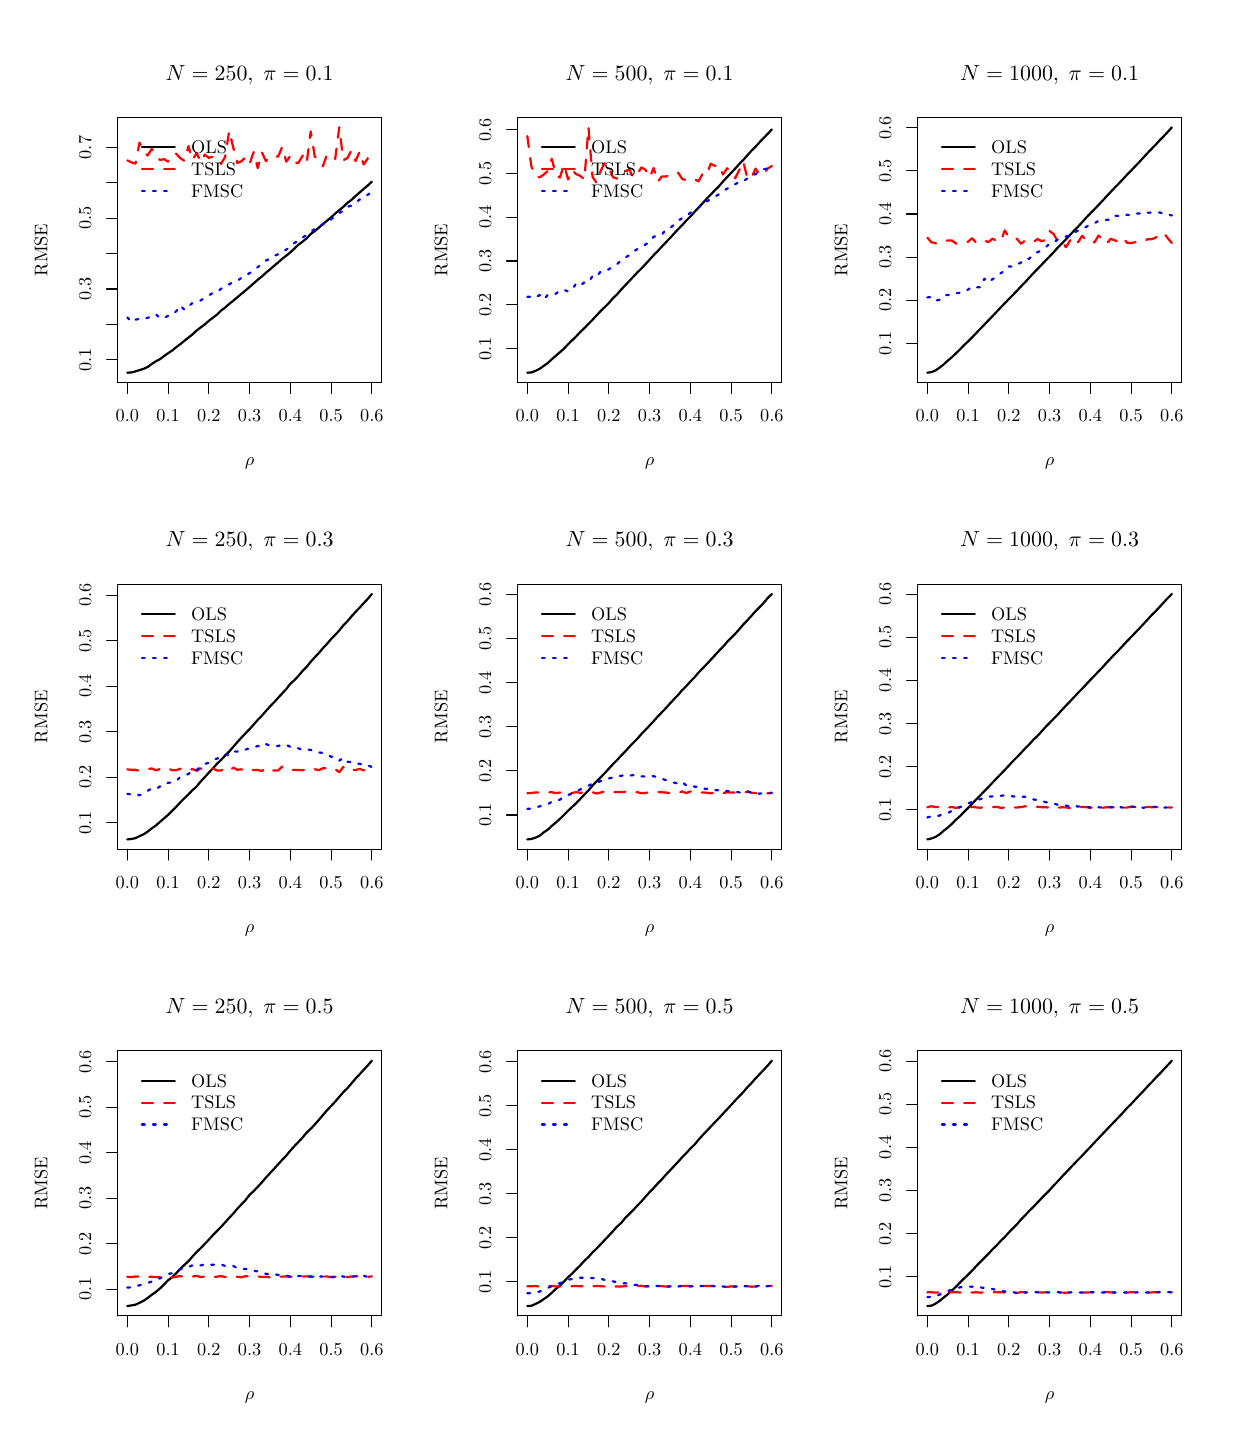
\begin{tikzpicture}[x=1pt,y=1pt]
\definecolor[named]{fillColor}{rgb}{1.00,1.00,1.00}
\path[use as bounding box,fill=fillColor,fill opacity=0.00] (0,0) rectangle (433.62,505.89);
\begin{scope}
\path[clip] ( 32.47,377.65) rectangle (127.91,473.42);
\definecolor[named]{drawColor}{rgb}{0.00,0.00,0.00}

\path[draw=drawColor,line width= 0.8pt,line join=round,line cap=round] ( 36.01,381.20) --
	( 37.48,381.31) --
	( 38.95,381.68) --
	( 40.42,382.15) --
	( 41.90,382.62) --
	( 43.37,383.28) --
	( 44.84,384.36) --
	( 46.32,385.32) --
	( 47.79,386.08) --
	( 49.26,387.20) --
	( 50.73,388.24) --
	( 52.21,389.21) --
	( 53.68,390.44) --
	( 55.15,391.53) --
	( 56.63,392.74) --
	( 58.10,393.92) --
	( 59.57,395.06) --
	( 61.04,396.45) --
	( 62.52,397.56) --
	( 63.99,398.65) --
	( 65.46,399.95) --
	( 66.93,401.10) --
	( 68.41,402.21) --
	( 69.88,403.65) --
	( 71.35,404.77) --
	( 72.83,406.06) --
	( 74.30,407.22) --
	( 75.77,408.48) --
	( 77.24,409.71) --
	( 78.72,410.94) --
	( 80.19,412.19) --
	( 81.66,413.47) --
	( 83.14,414.81) --
	( 84.61,415.96) --
	( 86.08,417.32) --
	( 87.55,418.51) --
	( 89.03,419.82) --
	( 90.50,421.04) --
	( 91.97,422.37) --
	( 93.44,423.48) --
	( 94.92,424.71) --
	( 96.39,426.08) --
	( 97.86,427.47) --
	( 99.34,428.57) --
	(100.81,429.76) --
	(102.28,431.34) --
	(103.75,432.41) --
	(105.23,433.63) --
	(106.70,434.96) --
	(108.17,436.12) --
	(109.65,437.35) --
	(111.12,438.70) --
	(112.59,439.94) --
	(114.06,441.14) --
	(115.54,442.56) --
	(117.01,443.66) --
	(118.48,445.05) --
	(119.95,446.32) --
	(121.43,447.63) --
	(122.90,448.86) --
	(124.37,450.23);
\end{scope}
\begin{scope}
\path[clip] (  0.00,  0.00) rectangle (433.62,505.89);
\definecolor[named]{drawColor}{rgb}{0.00,0.00,0.00}

\path[draw=drawColor,line width= 0.4pt,line join=round,line cap=round] ( 36.01,377.65) -- (124.37,377.65);

\path[draw=drawColor,line width= 0.4pt,line join=round,line cap=round] ( 36.01,377.65) -- ( 36.01,373.69);

\path[draw=drawColor,line width= 0.4pt,line join=round,line cap=round] ( 50.73,377.65) -- ( 50.73,373.69);

\path[draw=drawColor,line width= 0.4pt,line join=round,line cap=round] ( 65.46,377.65) -- ( 65.46,373.69);

\path[draw=drawColor,line width= 0.4pt,line join=round,line cap=round] ( 80.19,377.65) -- ( 80.19,373.69);

\path[draw=drawColor,line width= 0.4pt,line join=round,line cap=round] ( 94.92,377.65) -- ( 94.92,373.69);

\path[draw=drawColor,line width= 0.4pt,line join=round,line cap=round] (109.65,377.65) -- (109.65,373.69);

\path[draw=drawColor,line width= 0.4pt,line join=round,line cap=round] (124.37,377.65) -- (124.37,373.69);

\node[text=drawColor,anchor=base,inner sep=0pt, outer sep=0pt, scale=  0.66] at ( 36.01,363.40) {0.0};

\node[text=drawColor,anchor=base,inner sep=0pt, outer sep=0pt, scale=  0.66] at ( 50.73,363.40) {0.1};

\node[text=drawColor,anchor=base,inner sep=0pt, outer sep=0pt, scale=  0.66] at ( 65.46,363.40) {0.2};

\node[text=drawColor,anchor=base,inner sep=0pt, outer sep=0pt, scale=  0.66] at ( 80.19,363.40) {0.3};

\node[text=drawColor,anchor=base,inner sep=0pt, outer sep=0pt, scale=  0.66] at ( 94.92,363.40) {0.4};

\node[text=drawColor,anchor=base,inner sep=0pt, outer sep=0pt, scale=  0.66] at (109.65,363.40) {0.5};

\node[text=drawColor,anchor=base,inner sep=0pt, outer sep=0pt, scale=  0.66] at (124.37,363.40) {0.6};

\path[draw=drawColor,line width= 0.4pt,line join=round,line cap=round] ( 32.47,385.90) -- ( 32.47,462.60);

\path[draw=drawColor,line width= 0.4pt,line join=round,line cap=round] ( 32.47,385.90) -- ( 28.51,385.90);

\path[draw=drawColor,line width= 0.4pt,line join=round,line cap=round] ( 32.47,398.68) -- ( 28.51,398.68);

\path[draw=drawColor,line width= 0.4pt,line join=round,line cap=round] ( 32.47,411.46) -- ( 28.51,411.46);

\path[draw=drawColor,line width= 0.4pt,line join=round,line cap=round] ( 32.47,424.25) -- ( 28.51,424.25);

\path[draw=drawColor,line width= 0.4pt,line join=round,line cap=round] ( 32.47,437.03) -- ( 28.51,437.03);

\path[draw=drawColor,line width= 0.4pt,line join=round,line cap=round] ( 32.47,449.81) -- ( 28.51,449.81);

\path[draw=drawColor,line width= 0.4pt,line join=round,line cap=round] ( 32.47,462.60) -- ( 28.51,462.60);

\node[text=drawColor,rotate= 90.00,anchor=base,inner sep=0pt, outer sep=0pt, scale=  0.66] at ( 22.97,385.90) {0.1};

\node[text=drawColor,rotate= 90.00,anchor=base,inner sep=0pt, outer sep=0pt, scale=  0.66] at ( 22.97,411.46) {0.3};

\node[text=drawColor,rotate= 90.00,anchor=base,inner sep=0pt, outer sep=0pt, scale=  0.66] at ( 22.97,437.03) {0.5};

\node[text=drawColor,rotate= 90.00,anchor=base,inner sep=0pt, outer sep=0pt, scale=  0.66] at ( 22.97,462.60) {0.7};

\path[draw=drawColor,line width= 0.4pt,line join=round,line cap=round] ( 32.47,377.65) --
	(127.91,377.65) --
	(127.91,473.42) --
	( 32.47,473.42) --
	( 32.47,377.65);
\end{scope}
\begin{scope}
\path[clip] (  0.00,337.26) rectangle (144.54,505.89);
\definecolor[named]{drawColor}{rgb}{0.00,0.00,0.00}

\node[text=drawColor,anchor=base,inner sep=0pt, outer sep=0pt, scale=  0.79] at ( 80.19,486.92) {\bfseries $N=250, \;\pi=0.1$};

\node[text=drawColor,anchor=base,inner sep=0pt, outer sep=0pt, scale=  0.66] at ( 80.19,347.56) {$\rho$};

\node[text=drawColor,rotate= 90.00,anchor=base,inner sep=0pt, outer sep=0pt, scale=  0.66] at (  7.13,425.53) {RMSE};
\end{scope}
\begin{scope}
\path[clip] ( 32.47,377.65) rectangle (127.91,473.42);
\definecolor[named]{drawColor}{rgb}{1.00,0.00,0.00}

\path[draw=drawColor,line width= 0.8pt,dash pattern=on 4pt off 4pt ,line join=round,line cap=round] ( 36.01,457.95) --
	( 37.48,457.23) --
	( 38.95,456.75) --
	( 40.42,464.40) --
	( 41.90,460.96) --
	( 43.37,459.70) --
	( 44.84,462.07) --
	( 46.32,460.20) --
	( 47.79,458.06) --
	( 49.26,458.38) --
	( 50.73,457.46) --
	( 52.21,460.09) --
	( 53.68,460.32) --
	( 55.15,458.72) --
	( 56.63,457.75) --
	( 58.10,463.08) --
	( 59.57,458.02) --
	( 61.04,460.66) --
	( 62.52,457.29) --
	( 63.99,460.03) --
	( 65.46,458.82) --
	( 66.93,459.30) --
	( 68.41,459.00) --
	( 69.88,456.67) --
	( 71.35,459.20) --
	( 72.83,468.61) --
	( 74.30,462.50) --
	( 75.77,456.99) --
	( 77.24,457.61) --
	( 78.72,459.03) --
	( 80.19,456.60) --
	( 81.66,460.94) --
	( 83.14,455.16) --
	( 84.61,460.90) --
	( 86.08,457.66) --
	( 87.55,459.05) --
	( 89.03,459.65) --
	( 90.50,459.28) --
	( 91.97,462.79) --
	( 93.44,457.46) --
	( 94.92,459.60) --
	( 96.39,457.07) --
	( 97.86,457.06) --
	( 99.34,459.61) --
	(100.81,456.94) --
	(102.28,468.40) --
	(103.75,459.28) --
	(105.23,458.38) --
	(106.70,455.83) --
	(108.17,460.12) --
	(109.65,459.69) --
	(111.12,458.49) --
	(112.59,469.87) --
	(114.06,457.98) --
	(115.54,458.80) --
	(117.01,461.53) --
	(118.48,457.65) --
	(119.95,461.08) --
	(121.43,456.45) --
	(122.90,458.67) --
	(124.37,458.90);
\definecolor[named]{drawColor}{rgb}{0.00,0.00,1.00}

\path[draw=drawColor,line width= 0.8pt,dash pattern=on 1pt off 3pt ,line join=round,line cap=round] ( 36.01,401.23) --
	( 37.48,399.51) --
	( 38.95,400.37) --
	( 40.42,400.68) --
	( 41.90,400.58) --
	( 43.37,401.06) --
	( 44.84,401.50) --
	( 46.32,402.38) --
	( 47.79,400.86) --
	( 49.26,401.05) --
	( 50.73,401.72) --
	( 52.21,402.10) --
	( 53.68,403.44) --
	( 55.15,405.52) --
	( 56.63,403.92) --
	( 58.10,405.22) --
	( 59.57,406.39) --
	( 61.04,406.79) --
	( 62.52,407.29) --
	( 63.99,408.38) --
	( 65.46,409.16) --
	( 66.93,410.04) --
	( 68.41,410.28) --
	( 69.88,411.56) --
	( 71.35,412.21) --
	( 72.83,413.16) --
	( 74.30,414.05) --
	( 75.77,414.43) --
	( 77.24,415.48) --
	( 78.72,416.45) --
	( 80.19,417.20) --
	( 81.66,418.15) --
	( 83.14,419.36) --
	( 84.61,420.47) --
	( 86.08,421.71) --
	( 87.55,422.44) --
	( 89.03,423.38) --
	( 90.50,424.02) --
	( 91.97,425.01) --
	( 93.44,425.67) --
	( 94.92,426.78) --
	( 96.39,428.09) --
	( 97.86,429.00) --
	( 99.34,430.06) --
	(100.81,430.97) --
	(102.28,432.17) --
	(103.75,433.15) --
	(105.23,434.11) --
	(106.70,434.83) --
	(108.17,436.14) --
	(109.65,436.56) --
	(111.12,437.98) --
	(112.59,438.93) --
	(114.06,439.74) --
	(115.54,441.18) --
	(117.01,441.57) --
	(118.48,442.76) --
	(119.95,443.77) --
	(121.43,444.41) --
	(122.90,445.51) --
	(124.37,446.59);
\definecolor[named]{drawColor}{rgb}{0.00,0.00,0.00}

\path[draw=drawColor,line width= 0.8pt,line join=round,line cap=round] ( 41.28,462.63) -- ( 53.16,462.63);
\definecolor[named]{drawColor}{rgb}{1.00,0.00,0.00}

\path[draw=drawColor,line width= 0.8pt,dash pattern=on 4pt off 4pt ,line join=round,line cap=round] ( 41.28,454.71) -- ( 53.16,454.71);
\definecolor[named]{drawColor}{rgb}{0.00,0.00,1.00}

\path[draw=drawColor,line width= 0.8pt,dash pattern=on 1pt off 3pt ,line join=round,line cap=round] ( 41.28,446.79) -- ( 53.16,446.79);
\definecolor[named]{drawColor}{rgb}{0.00,0.00,0.00}

\node[text=drawColor,anchor=base west,inner sep=0pt, outer sep=0pt, scale=  0.66] at ( 59.10,460.35) {OLS};

\node[text=drawColor,anchor=base west,inner sep=0pt, outer sep=0pt, scale=  0.66] at ( 59.10,452.43) {TSLS};

\node[text=drawColor,anchor=base west,inner sep=0pt, outer sep=0pt, scale=  0.66] at ( 59.10,444.51) {FMSC};
\end{scope}
\begin{scope}
\path[clip] (177.01,377.65) rectangle (272.45,473.42);
\definecolor[named]{drawColor}{rgb}{0.00,0.00,0.00}

\path[draw=drawColor,line width= 0.8pt,line join=round,line cap=round] (180.55,381.20) --
	(182.02,381.31) --
	(183.49,381.86) --
	(184.96,382.60) --
	(186.44,383.64) --
	(187.91,384.69) --
	(189.38,386.05) --
	(190.86,387.35) --
	(192.33,388.61) --
	(193.80,389.91) --
	(195.27,391.49) --
	(196.75,392.93) --
	(198.22,394.33) --
	(199.69,395.94) --
	(201.17,397.31) --
	(202.64,398.85) --
	(204.11,400.33) --
	(205.58,401.90) --
	(207.06,403.51) --
	(208.53,404.92) --
	(210.00,406.39) --
	(211.47,408.09) --
	(212.95,409.49) --
	(214.42,411.19) --
	(215.89,412.76) --
	(217.37,414.30) --
	(218.84,415.87) --
	(220.31,417.45) --
	(221.78,418.87) --
	(223.26,420.47) --
	(224.73,422.05) --
	(226.20,423.70) --
	(227.68,425.16) --
	(229.15,426.77) --
	(230.62,428.32) --
	(232.09,429.84) --
	(233.57,431.48) --
	(235.04,433.06) --
	(236.51,434.55) --
	(237.98,436.16) --
	(239.46,437.64) --
	(240.93,439.28) --
	(242.40,440.84) --
	(243.88,442.42) --
	(245.35,444.06) --
	(246.82,445.54) --
	(248.29,447.10) --
	(249.77,448.55) --
	(251.24,450.29) --
	(252.71,451.85) --
	(254.19,453.41) --
	(255.66,454.98) --
	(257.13,456.61) --
	(258.60,458.10) --
	(260.08,459.78) --
	(261.55,461.44) --
	(263.02,462.86) --
	(264.50,464.51) --
	(265.97,466.07) --
	(267.44,467.55) --
	(268.91,469.15);
\end{scope}
\begin{scope}
\path[clip] (  0.00,  0.00) rectangle (433.62,505.89);
\definecolor[named]{drawColor}{rgb}{0.00,0.00,0.00}

\path[draw=drawColor,line width= 0.4pt,line join=round,line cap=round] (180.55,377.65) -- (268.91,377.65);

\path[draw=drawColor,line width= 0.4pt,line join=round,line cap=round] (180.55,377.65) -- (180.55,373.69);

\path[draw=drawColor,line width= 0.4pt,line join=round,line cap=round] (195.27,377.65) -- (195.27,373.69);

\path[draw=drawColor,line width= 0.4pt,line join=round,line cap=round] (210.00,377.65) -- (210.00,373.69);

\path[draw=drawColor,line width= 0.4pt,line join=round,line cap=round] (224.73,377.65) -- (224.73,373.69);

\path[draw=drawColor,line width= 0.4pt,line join=round,line cap=round] (239.46,377.65) -- (239.46,373.69);

\path[draw=drawColor,line width= 0.4pt,line join=round,line cap=round] (254.19,377.65) -- (254.19,373.69);

\path[draw=drawColor,line width= 0.4pt,line join=round,line cap=round] (268.91,377.65) -- (268.91,373.69);

\node[text=drawColor,anchor=base,inner sep=0pt, outer sep=0pt, scale=  0.66] at (180.55,363.40) {0.0};

\node[text=drawColor,anchor=base,inner sep=0pt, outer sep=0pt, scale=  0.66] at (195.27,363.40) {0.1};

\node[text=drawColor,anchor=base,inner sep=0pt, outer sep=0pt, scale=  0.66] at (210.00,363.40) {0.2};

\node[text=drawColor,anchor=base,inner sep=0pt, outer sep=0pt, scale=  0.66] at (224.73,363.40) {0.3};

\node[text=drawColor,anchor=base,inner sep=0pt, outer sep=0pt, scale=  0.66] at (239.46,363.40) {0.4};

\node[text=drawColor,anchor=base,inner sep=0pt, outer sep=0pt, scale=  0.66] at (254.19,363.40) {0.5};

\node[text=drawColor,anchor=base,inner sep=0pt, outer sep=0pt, scale=  0.66] at (268.91,363.40) {0.6};

\path[draw=drawColor,line width= 0.4pt,line join=round,line cap=round] (177.01,389.93) -- (177.01,469.01);

\path[draw=drawColor,line width= 0.4pt,line join=round,line cap=round] (177.01,389.93) -- (173.05,389.93);

\path[draw=drawColor,line width= 0.4pt,line join=round,line cap=round] (177.01,405.74) -- (173.05,405.74);

\path[draw=drawColor,line width= 0.4pt,line join=round,line cap=round] (177.01,421.56) -- (173.05,421.56);

\path[draw=drawColor,line width= 0.4pt,line join=round,line cap=round] (177.01,437.38) -- (173.05,437.38);

\path[draw=drawColor,line width= 0.4pt,line join=round,line cap=round] (177.01,453.19) -- (173.05,453.19);

\path[draw=drawColor,line width= 0.4pt,line join=round,line cap=round] (177.01,469.01) -- (173.05,469.01);

\node[text=drawColor,rotate= 90.00,anchor=base,inner sep=0pt, outer sep=0pt, scale=  0.66] at (167.51,389.93) {0.1};

\node[text=drawColor,rotate= 90.00,anchor=base,inner sep=0pt, outer sep=0pt, scale=  0.66] at (167.51,405.74) {0.2};

\node[text=drawColor,rotate= 90.00,anchor=base,inner sep=0pt, outer sep=0pt, scale=  0.66] at (167.51,421.56) {0.3};

\node[text=drawColor,rotate= 90.00,anchor=base,inner sep=0pt, outer sep=0pt, scale=  0.66] at (167.51,437.38) {0.4};

\node[text=drawColor,rotate= 90.00,anchor=base,inner sep=0pt, outer sep=0pt, scale=  0.66] at (167.51,453.19) {0.5};

\node[text=drawColor,rotate= 90.00,anchor=base,inner sep=0pt, outer sep=0pt, scale=  0.66] at (167.51,469.01) {0.6};

\path[draw=drawColor,line width= 0.4pt,line join=round,line cap=round] (177.01,377.65) --
	(272.45,377.65) --
	(272.45,473.42) --
	(177.01,473.42) --
	(177.01,377.65);
\end{scope}
\begin{scope}
\path[clip] (144.54,337.26) rectangle (289.08,505.89);
\definecolor[named]{drawColor}{rgb}{0.00,0.00,0.00}

\node[text=drawColor,anchor=base,inner sep=0pt, outer sep=0pt, scale=  0.79] at (224.73,486.92) {\bfseries $N=500, \;\pi=0.1$};

\node[text=drawColor,anchor=base,inner sep=0pt, outer sep=0pt, scale=  0.66] at (224.73,347.56) {$\rho$};

\node[text=drawColor,rotate= 90.00,anchor=base,inner sep=0pt, outer sep=0pt, scale=  0.66] at (151.67,425.53) {RMSE};
\end{scope}
\begin{scope}
\path[clip] (177.01,377.65) rectangle (272.45,473.42);
\definecolor[named]{drawColor}{rgb}{1.00,0.00,0.00}

\path[draw=drawColor,line width= 0.8pt,dash pattern=on 4pt off 4pt ,line join=round,line cap=round] (180.55,466.72) --
	(182.02,455.74) --
	(183.49,452.28) --
	(184.96,451.80) --
	(186.44,452.78) --
	(187.91,454.08) --
	(189.38,458.54) --
	(190.86,452.70) --
	(192.33,451.73) --
	(193.80,456.48) --
	(195.27,451.04) --
	(196.75,454.48) --
	(198.22,452.92) --
	(199.69,452.35) --
	(201.17,450.95) --
	(202.64,469.87) --
	(204.11,451.98) --
	(205.58,449.82) --
	(207.06,454.09) --
	(208.53,457.15) --
	(210.00,455.29) --
	(211.47,451.89) --
	(212.95,451.34) --
	(214.42,453.57) --
	(215.89,454.06) --
	(217.37,454.59) --
	(218.84,451.70) --
	(220.31,453.03) --
	(221.78,455.41) --
	(223.26,454.53) --
	(224.73,451.76) --
	(226.20,455.17) --
	(227.68,450.17) --
	(229.15,452.12) --
	(230.62,452.05) --
	(232.09,452.77) --
	(233.57,452.63) --
	(235.04,453.52) --
	(236.51,451.22) --
	(237.98,450.77) --
	(239.46,451.21) --
	(240.93,451.13) --
	(242.40,450.37) --
	(243.88,453.05) --
	(245.35,452.60) --
	(246.82,456.72) --
	(248.29,455.97) --
	(249.77,456.22) --
	(251.24,452.84) --
	(252.71,455.06) --
	(254.19,454.01) --
	(255.66,451.46) --
	(257.13,454.41) --
	(258.60,457.49) --
	(260.08,451.34) --
	(261.55,451.78) --
	(263.02,454.96) --
	(264.50,452.70) --
	(265.97,453.02) --
	(267.44,455.04) --
	(268.91,455.88);
\definecolor[named]{drawColor}{rgb}{0.00,0.00,1.00}

\path[draw=drawColor,line width= 0.8pt,dash pattern=on 1pt off 3pt ,line join=round,line cap=round] (180.55,408.62) --
	(182.02,408.70) --
	(183.49,408.29) --
	(184.96,409.27) --
	(186.44,407.70) --
	(187.91,409.28) --
	(189.38,409.87) --
	(190.86,409.74) --
	(192.33,411.06) --
	(193.80,411.13) --
	(195.27,410.58) --
	(196.75,411.25) --
	(198.22,413.50) --
	(199.69,412.72) --
	(201.17,413.86) --
	(202.64,413.80) --
	(204.11,416.17) --
	(205.58,415.89) --
	(207.06,417.80) --
	(208.53,417.86) --
	(210.00,418.58) --
	(211.47,419.59) --
	(212.95,420.41) --
	(214.42,421.78) --
	(215.89,422.84) --
	(217.37,423.63) --
	(218.84,424.92) --
	(220.31,425.87) --
	(221.78,426.51) --
	(223.26,427.57) --
	(224.73,428.44) --
	(226.20,430.34) --
	(227.68,430.70) --
	(229.15,431.08) --
	(230.62,432.93) --
	(232.09,433.47) --
	(233.57,434.66) --
	(235.04,436.09) --
	(236.51,437.10) --
	(237.98,437.72) --
	(239.46,439.02) --
	(240.93,439.77) --
	(242.40,440.86) --
	(243.88,442.22) --
	(245.35,443.13) --
	(246.82,443.89) --
	(248.29,444.81) --
	(249.77,445.67) --
	(251.24,446.76) --
	(252.71,447.72) --
	(254.19,448.30) --
	(255.66,449.32) --
	(257.13,450.22) --
	(258.60,450.35) --
	(260.08,451.46) --
	(261.55,452.36) --
	(263.02,452.95) --
	(264.50,454.18) --
	(265.97,454.74) --
	(267.44,454.96) --
	(268.91,455.83);
\definecolor[named]{drawColor}{rgb}{0.00,0.00,0.00}

\path[draw=drawColor,line width= 0.8pt,line join=round,line cap=round] (185.82,462.63) -- (197.70,462.63);
\definecolor[named]{drawColor}{rgb}{1.00,0.00,0.00}

\path[draw=drawColor,line width= 0.8pt,dash pattern=on 4pt off 4pt ,line join=round,line cap=round] (185.82,454.71) -- (197.70,454.71);
\definecolor[named]{drawColor}{rgb}{0.00,0.00,1.00}

\path[draw=drawColor,line width= 0.8pt,dash pattern=on 1pt off 3pt ,line join=round,line cap=round] (185.82,446.79) -- (197.70,446.79);
\definecolor[named]{drawColor}{rgb}{0.00,0.00,0.00}

\node[text=drawColor,anchor=base west,inner sep=0pt, outer sep=0pt, scale=  0.66] at (203.64,460.35) {OLS};

\node[text=drawColor,anchor=base west,inner sep=0pt, outer sep=0pt, scale=  0.66] at (203.64,452.43) {TSLS};

\node[text=drawColor,anchor=base west,inner sep=0pt, outer sep=0pt, scale=  0.66] at (203.64,444.51) {FMSC};
\end{scope}
\begin{scope}
\path[clip] (321.55,377.65) rectangle (416.99,473.42);
\definecolor[named]{drawColor}{rgb}{0.00,0.00,0.00}

\path[draw=drawColor,line width= 0.8pt,line join=round,line cap=round] (325.09,381.20) --
	(326.56,381.41) --
	(328.03,382.02) --
	(329.50,383.03) --
	(330.98,384.18) --
	(332.45,385.54) --
	(333.92,386.78) --
	(335.40,388.19) --
	(336.87,389.60) --
	(338.34,391.14) --
	(339.81,392.51) --
	(341.29,394.00) --
	(342.76,395.54) --
	(344.23,397.07) --
	(345.71,398.61) --
	(347.18,400.14) --
	(348.65,401.63) --
	(350.12,403.22) --
	(351.60,404.78) --
	(353.07,406.31) --
	(354.54,407.83) --
	(356.01,409.31) --
	(357.49,410.83) --
	(358.96,412.41) --
	(360.43,413.91) --
	(361.91,415.52) --
	(363.38,417.12) --
	(364.85,418.65) --
	(366.32,420.15) --
	(367.80,421.71) --
	(369.27,423.21) --
	(370.74,424.75) --
	(372.22,426.41) --
	(373.69,427.86) --
	(375.16,429.38) --
	(376.63,430.99) --
	(378.11,432.53) --
	(379.58,434.01) --
	(381.05,435.61) --
	(382.52,437.26) --
	(384.00,438.78) --
	(385.47,440.27) --
	(386.94,441.81) --
	(388.42,443.37) --
	(389.89,444.98) --
	(391.36,446.54) --
	(392.83,448.11) --
	(394.31,449.61) --
	(395.78,451.15) --
	(397.25,452.74) --
	(398.73,454.23) --
	(400.20,455.80) --
	(401.67,457.32) --
	(403.14,458.94) --
	(404.62,460.53) --
	(406.09,462.06) --
	(407.56,463.56) --
	(409.04,465.17) --
	(410.51,466.66) --
	(411.98,468.24) --
	(413.45,469.87);
\end{scope}
\begin{scope}
\path[clip] (  0.00,  0.00) rectangle (433.62,505.89);
\definecolor[named]{drawColor}{rgb}{0.00,0.00,0.00}

\path[draw=drawColor,line width= 0.4pt,line join=round,line cap=round] (325.09,377.65) -- (413.45,377.65);

\path[draw=drawColor,line width= 0.4pt,line join=round,line cap=round] (325.09,377.65) -- (325.09,373.69);

\path[draw=drawColor,line width= 0.4pt,line join=round,line cap=round] (339.81,377.65) -- (339.81,373.69);

\path[draw=drawColor,line width= 0.4pt,line join=round,line cap=round] (354.54,377.65) -- (354.54,373.69);

\path[draw=drawColor,line width= 0.4pt,line join=round,line cap=round] (369.27,377.65) -- (369.27,373.69);

\path[draw=drawColor,line width= 0.4pt,line join=round,line cap=round] (384.00,377.65) -- (384.00,373.69);

\path[draw=drawColor,line width= 0.4pt,line join=round,line cap=round] (398.73,377.65) -- (398.73,373.69);

\path[draw=drawColor,line width= 0.4pt,line join=round,line cap=round] (413.45,377.65) -- (413.45,373.69);

\node[text=drawColor,anchor=base,inner sep=0pt, outer sep=0pt, scale=  0.66] at (325.09,363.40) {0.0};

\node[text=drawColor,anchor=base,inner sep=0pt, outer sep=0pt, scale=  0.66] at (339.81,363.40) {0.1};

\node[text=drawColor,anchor=base,inner sep=0pt, outer sep=0pt, scale=  0.66] at (354.54,363.40) {0.2};

\node[text=drawColor,anchor=base,inner sep=0pt, outer sep=0pt, scale=  0.66] at (369.27,363.40) {0.3};

\node[text=drawColor,anchor=base,inner sep=0pt, outer sep=0pt, scale=  0.66] at (384.00,363.40) {0.4};

\node[text=drawColor,anchor=base,inner sep=0pt, outer sep=0pt, scale=  0.66] at (398.73,363.40) {0.5};

\node[text=drawColor,anchor=base,inner sep=0pt, outer sep=0pt, scale=  0.66] at (413.45,363.40) {0.6};

\path[draw=drawColor,line width= 0.4pt,line join=round,line cap=round] (321.55,391.81) -- (321.55,469.74);

\path[draw=drawColor,line width= 0.4pt,line join=round,line cap=round] (321.55,391.81) -- (317.59,391.81);

\path[draw=drawColor,line width= 0.4pt,line join=round,line cap=round] (321.55,407.40) -- (317.59,407.40);

\path[draw=drawColor,line width= 0.4pt,line join=round,line cap=round] (321.55,422.98) -- (317.59,422.98);

\path[draw=drawColor,line width= 0.4pt,line join=round,line cap=round] (321.55,438.57) -- (317.59,438.57);

\path[draw=drawColor,line width= 0.4pt,line join=round,line cap=round] (321.55,454.15) -- (317.59,454.15);

\path[draw=drawColor,line width= 0.4pt,line join=round,line cap=round] (321.55,469.74) -- (317.59,469.74);

\node[text=drawColor,rotate= 90.00,anchor=base,inner sep=0pt, outer sep=0pt, scale=  0.66] at (312.05,391.81) {0.1};

\node[text=drawColor,rotate= 90.00,anchor=base,inner sep=0pt, outer sep=0pt, scale=  0.66] at (312.05,407.40) {0.2};

\node[text=drawColor,rotate= 90.00,anchor=base,inner sep=0pt, outer sep=0pt, scale=  0.66] at (312.05,422.98) {0.3};

\node[text=drawColor,rotate= 90.00,anchor=base,inner sep=0pt, outer sep=0pt, scale=  0.66] at (312.05,438.57) {0.4};

\node[text=drawColor,rotate= 90.00,anchor=base,inner sep=0pt, outer sep=0pt, scale=  0.66] at (312.05,454.15) {0.5};

\node[text=drawColor,rotate= 90.00,anchor=base,inner sep=0pt, outer sep=0pt, scale=  0.66] at (312.05,469.74) {0.6};

\path[draw=drawColor,line width= 0.4pt,line join=round,line cap=round] (321.55,377.65) --
	(416.99,377.65) --
	(416.99,473.42) --
	(321.55,473.42) --
	(321.55,377.65);
\end{scope}
\begin{scope}
\path[clip] (289.08,337.26) rectangle (433.62,505.89);
\definecolor[named]{drawColor}{rgb}{0.00,0.00,0.00}

\node[text=drawColor,anchor=base,inner sep=0pt, outer sep=0pt, scale=  0.79] at (369.27,486.92) {\bfseries $N=1000, \;\pi=0.1$};

\node[text=drawColor,anchor=base,inner sep=0pt, outer sep=0pt, scale=  0.66] at (369.27,347.56) {$\rho$};

\node[text=drawColor,rotate= 90.00,anchor=base,inner sep=0pt, outer sep=0pt, scale=  0.66] at (296.21,425.53) {RMSE};
\end{scope}
\begin{scope}
\path[clip] (321.55,377.65) rectangle (416.99,473.42);
\definecolor[named]{drawColor}{rgb}{1.00,0.00,0.00}

\path[draw=drawColor,line width= 0.8pt,dash pattern=on 4pt off 4pt ,line join=round,line cap=round] (325.09,430.04) --
	(326.56,428.32) --
	(328.03,428.02) --
	(329.50,427.94) --
	(330.98,428.70) --
	(332.45,428.97) --
	(333.92,429.02) --
	(335.40,427.90) --
	(336.87,428.16) --
	(338.34,428.02) --
	(339.81,428.56) --
	(341.29,429.80) --
	(342.76,428.13) --
	(344.23,428.50) --
	(345.71,428.94) --
	(347.18,428.41) --
	(348.65,429.64) --
	(350.12,428.91) --
	(351.60,428.64) --
	(353.07,432.61) --
	(354.54,430.18) --
	(356.01,429.93) --
	(357.49,429.55) --
	(358.96,427.80) --
	(360.43,428.95) --
	(361.91,428.44) --
	(363.38,428.30) --
	(364.85,429.51) --
	(366.32,428.77) --
	(367.80,429.12) --
	(369.27,432.39) --
	(370.74,431.30) --
	(372.22,428.67) --
	(373.69,428.68) --
	(375.16,426.55) --
	(376.63,428.89) --
	(378.11,430.27) --
	(379.58,428.39) --
	(381.05,430.68) --
	(382.52,429.00) --
	(384.00,429.21) --
	(385.47,428.27) --
	(386.94,430.74) --
	(388.42,429.51) --
	(389.89,427.82) --
	(391.36,429.62) --
	(392.83,429.01) --
	(394.31,428.68) --
	(395.78,429.85) --
	(397.25,428.20) --
	(398.73,428.05) --
	(400.20,428.38) --
	(401.67,428.55) --
	(403.14,428.64) --
	(404.62,429.41) --
	(406.09,429.42) --
	(407.56,430.00) --
	(409.04,430.97) --
	(410.51,431.73) --
	(411.98,429.82) --
	(413.45,428.07);
\definecolor[named]{drawColor}{rgb}{0.00,0.00,1.00}

\path[draw=drawColor,line width= 0.8pt,dash pattern=on 1pt off 3pt ,line join=round,line cap=round] (325.09,408.41) --
	(326.56,408.54) --
	(328.03,407.24) --
	(329.50,407.57) --
	(330.98,409.15) --
	(332.45,409.29) --
	(333.92,409.25) --
	(335.40,409.92) --
	(336.87,410.08) --
	(338.34,410.55) --
	(339.81,411.24) --
	(341.29,412.36) --
	(342.76,412.06) --
	(344.23,412.08) --
	(345.71,415.16) --
	(347.18,413.79) --
	(348.65,415.04) --
	(350.12,415.73) --
	(351.60,417.19) --
	(353.07,417.97) --
	(354.54,419.60) --
	(356.01,419.54) --
	(357.49,420.31) --
	(358.96,421.02) --
	(360.43,422.38) --
	(361.91,422.39) --
	(363.38,424.05) --
	(364.85,424.72) --
	(366.32,425.42) --
	(367.80,426.46) --
	(369.27,427.87) --
	(370.74,428.21) --
	(372.22,429.35) --
	(373.69,429.90) --
	(375.16,430.39) --
	(376.63,430.84) --
	(378.11,431.81) --
	(379.58,432.59) --
	(381.05,433.45) --
	(382.52,433.91) --
	(384.00,434.80) --
	(385.47,435.19) --
	(386.94,436.09) --
	(388.42,436.30) --
	(389.89,436.44) --
	(391.36,436.60) --
	(392.83,437.92) --
	(394.31,437.85) --
	(395.78,437.68) --
	(397.25,438.28) --
	(398.73,438.08) --
	(400.20,438.61) --
	(401.67,438.79) --
	(403.14,438.58) --
	(404.62,439.02) --
	(406.09,439.07) --
	(407.56,439.07) --
	(409.04,439.10) --
	(410.51,438.72) --
	(411.98,438.40) --
	(413.45,438.03);
\definecolor[named]{drawColor}{rgb}{0.00,0.00,0.00}

\path[draw=drawColor,line width= 0.8pt,line join=round,line cap=round] (330.36,462.63) -- (342.24,462.63);
\definecolor[named]{drawColor}{rgb}{1.00,0.00,0.00}

\path[draw=drawColor,line width= 0.8pt,dash pattern=on 4pt off 4pt ,line join=round,line cap=round] (330.36,454.71) -- (342.24,454.71);
\definecolor[named]{drawColor}{rgb}{0.00,0.00,1.00}

\path[draw=drawColor,line width= 0.8pt,dash pattern=on 1pt off 3pt ,line join=round,line cap=round] (330.36,446.79) -- (342.24,446.79);
\definecolor[named]{drawColor}{rgb}{0.00,0.00,0.00}

\node[text=drawColor,anchor=base west,inner sep=0pt, outer sep=0pt, scale=  0.66] at (348.18,460.35) {OLS};

\node[text=drawColor,anchor=base west,inner sep=0pt, outer sep=0pt, scale=  0.66] at (348.18,452.43) {TSLS};

\node[text=drawColor,anchor=base west,inner sep=0pt, outer sep=0pt, scale=  0.66] at (348.18,444.51) {FMSC};
\end{scope}
\begin{scope}
\path[clip] ( 32.47,209.02) rectangle (127.91,304.79);
\definecolor[named]{drawColor}{rgb}{0.00,0.00,0.00}

\path[draw=drawColor,line width= 0.8pt,line join=round,line cap=round] ( 36.01,212.57) --
	( 37.48,212.71) --
	( 38.95,213.03) --
	( 40.42,213.76) --
	( 41.90,214.43) --
	( 43.37,215.41) --
	( 44.84,216.56) --
	( 46.32,217.59) --
	( 47.79,218.89) --
	( 49.26,220.16) --
	( 50.73,221.41) --
	( 52.21,222.89) --
	( 53.68,224.37) --
	( 55.15,225.95) --
	( 56.63,227.43) --
	( 58.10,228.84) --
	( 59.57,230.39) --
	( 61.04,231.65) --
	( 62.52,233.52) --
	( 63.99,235.04) --
	( 65.46,236.69) --
	( 66.93,238.23) --
	( 68.41,239.91) --
	( 69.88,241.29) --
	( 71.35,242.84) --
	( 72.83,244.32) --
	( 74.30,246.01) --
	( 75.77,247.75) --
	( 77.24,249.35) --
	( 78.72,250.92) --
	( 80.19,252.40) --
	( 81.66,254.06) --
	( 83.14,255.75) --
	( 84.61,257.23) --
	( 86.08,258.94) --
	( 87.55,260.59) --
	( 89.03,262.10) --
	( 90.50,263.74) --
	( 91.97,265.31) --
	( 93.44,266.88) --
	( 94.92,268.83) --
	( 96.39,270.11) --
	( 97.86,271.67) --
	( 99.34,273.45) --
	(100.81,274.94) --
	(102.28,276.76) --
	(103.75,278.38) --
	(105.23,279.94) --
	(106.70,281.69) --
	(108.17,283.23) --
	(109.65,284.98) --
	(111.12,286.48) --
	(112.59,288.05) --
	(114.06,289.89) --
	(115.54,291.40) --
	(117.01,293.17) --
	(118.48,294.75) --
	(119.95,296.30) --
	(121.43,297.93) --
	(122.90,299.50) --
	(124.37,301.24);
\end{scope}
\begin{scope}
\path[clip] (  0.00,  0.00) rectangle (433.62,505.89);
\definecolor[named]{drawColor}{rgb}{0.00,0.00,0.00}

\path[draw=drawColor,line width= 0.4pt,line join=round,line cap=round] ( 36.01,209.02) -- (124.37,209.02);

\path[draw=drawColor,line width= 0.4pt,line join=round,line cap=round] ( 36.01,209.02) -- ( 36.01,205.06);

\path[draw=drawColor,line width= 0.4pt,line join=round,line cap=round] ( 50.73,209.02) -- ( 50.73,205.06);

\path[draw=drawColor,line width= 0.4pt,line join=round,line cap=round] ( 65.46,209.02) -- ( 65.46,205.06);

\path[draw=drawColor,line width= 0.4pt,line join=round,line cap=round] ( 80.19,209.02) -- ( 80.19,205.06);

\path[draw=drawColor,line width= 0.4pt,line join=round,line cap=round] ( 94.92,209.02) -- ( 94.92,205.06);

\path[draw=drawColor,line width= 0.4pt,line join=round,line cap=round] (109.65,209.02) -- (109.65,205.06);

\path[draw=drawColor,line width= 0.4pt,line join=round,line cap=round] (124.37,209.02) -- (124.37,205.06);

\node[text=drawColor,anchor=base,inner sep=0pt, outer sep=0pt, scale=  0.66] at ( 36.01,194.77) {0.0};

\node[text=drawColor,anchor=base,inner sep=0pt, outer sep=0pt, scale=  0.66] at ( 50.73,194.77) {0.1};

\node[text=drawColor,anchor=base,inner sep=0pt, outer sep=0pt, scale=  0.66] at ( 65.46,194.77) {0.2};

\node[text=drawColor,anchor=base,inner sep=0pt, outer sep=0pt, scale=  0.66] at ( 80.19,194.77) {0.3};

\node[text=drawColor,anchor=base,inner sep=0pt, outer sep=0pt, scale=  0.66] at ( 94.92,194.77) {0.4};

\node[text=drawColor,anchor=base,inner sep=0pt, outer sep=0pt, scale=  0.66] at (109.65,194.77) {0.5};

\node[text=drawColor,anchor=base,inner sep=0pt, outer sep=0pt, scale=  0.66] at (124.37,194.77) {0.6};

\path[draw=drawColor,line width= 0.4pt,line join=round,line cap=round] ( 32.47,218.58) -- ( 32.47,300.82);

\path[draw=drawColor,line width= 0.4pt,line join=round,line cap=round] ( 32.47,218.58) -- ( 28.51,218.58);

\path[draw=drawColor,line width= 0.4pt,line join=round,line cap=round] ( 32.47,235.03) -- ( 28.51,235.03);

\path[draw=drawColor,line width= 0.4pt,line join=round,line cap=round] ( 32.47,251.48) -- ( 28.51,251.48);

\path[draw=drawColor,line width= 0.4pt,line join=round,line cap=round] ( 32.47,267.93) -- ( 28.51,267.93);

\path[draw=drawColor,line width= 0.4pt,line join=round,line cap=round] ( 32.47,284.37) -- ( 28.51,284.37);

\path[draw=drawColor,line width= 0.4pt,line join=round,line cap=round] ( 32.47,300.82) -- ( 28.51,300.82);

\node[text=drawColor,rotate= 90.00,anchor=base,inner sep=0pt, outer sep=0pt, scale=  0.66] at ( 22.97,218.58) {0.1};

\node[text=drawColor,rotate= 90.00,anchor=base,inner sep=0pt, outer sep=0pt, scale=  0.66] at ( 22.97,235.03) {0.2};

\node[text=drawColor,rotate= 90.00,anchor=base,inner sep=0pt, outer sep=0pt, scale=  0.66] at ( 22.97,251.48) {0.3};

\node[text=drawColor,rotate= 90.00,anchor=base,inner sep=0pt, outer sep=0pt, scale=  0.66] at ( 22.97,267.93) {0.4};

\node[text=drawColor,rotate= 90.00,anchor=base,inner sep=0pt, outer sep=0pt, scale=  0.66] at ( 22.97,284.37) {0.5};

\node[text=drawColor,rotate= 90.00,anchor=base,inner sep=0pt, outer sep=0pt, scale=  0.66] at ( 22.97,300.82) {0.6};

\path[draw=drawColor,line width= 0.4pt,line join=round,line cap=round] ( 32.47,209.02) --
	(127.91,209.02) --
	(127.91,304.79) --
	( 32.47,304.79) --
	( 32.47,209.02);
\end{scope}
\begin{scope}
\path[clip] (  0.00,168.63) rectangle (144.54,337.26);
\definecolor[named]{drawColor}{rgb}{0.00,0.00,0.00}

\node[text=drawColor,anchor=base,inner sep=0pt, outer sep=0pt, scale=  0.79] at ( 80.19,318.29) {\bfseries $N=250, \;\pi=0.3$};

\node[text=drawColor,anchor=base,inner sep=0pt, outer sep=0pt, scale=  0.66] at ( 80.19,178.93) {$\rho$};

\node[text=drawColor,rotate= 90.00,anchor=base,inner sep=0pt, outer sep=0pt, scale=  0.66] at (  7.13,256.90) {RMSE};
\end{scope}
\begin{scope}
\path[clip] ( 32.47,209.02) rectangle (127.91,304.79);
\definecolor[named]{drawColor}{rgb}{1.00,0.00,0.00}

\path[draw=drawColor,line width= 0.8pt,dash pattern=on 4pt off 4pt ,line join=round,line cap=round] ( 36.01,237.89) --
	( 37.48,237.71) --
	( 38.95,237.72) --
	( 40.42,237.34) --
	( 41.90,237.67) --
	( 43.37,237.93) --
	( 44.84,238.20) --
	( 46.32,237.55) --
	( 47.79,237.98) --
	( 49.26,237.75) --
	( 50.73,238.25) --
	( 52.21,237.54) --
	( 53.68,237.58) --
	( 55.15,238.09) --
	( 56.63,237.49) --
	( 58.10,237.47) --
	( 59.57,237.99) --
	( 61.04,237.36) --
	( 62.52,238.20) --
	( 63.99,237.78) --
	( 65.46,237.74) --
	( 66.93,238.26) --
	( 68.41,237.48) --
	( 69.88,237.44) --
	( 71.35,238.17) --
	( 72.83,237.41) --
	( 74.30,238.48) --
	( 75.77,237.73) --
	( 77.24,237.90) --
	( 78.72,237.25) --
	( 80.19,237.62) --
	( 81.66,237.64) --
	( 83.14,237.70) --
	( 84.61,237.24) --
	( 86.08,238.41) --
	( 87.55,237.74) --
	( 89.03,237.45) --
	( 90.50,237.47) --
	( 91.97,238.88) --
	( 93.44,238.06) --
	( 94.92,237.55) --
	( 96.39,237.70) --
	( 97.86,237.66) --
	( 99.34,237.56) --
	(100.81,237.97) --
	(102.28,237.83) --
	(103.75,237.91) --
	(105.23,237.63) --
	(106.70,238.29) --
	(108.17,238.27) --
	(109.65,237.87) --
	(111.12,237.95) --
	(112.59,236.86) --
	(114.06,238.75) --
	(115.54,237.53) --
	(117.01,237.76) --
	(118.48,237.63) --
	(119.95,238.06) --
	(121.43,237.54) --
	(122.90,237.93) --
	(124.37,237.53);
\definecolor[named]{drawColor}{rgb}{0.00,0.00,1.00}

\path[draw=drawColor,line width= 0.8pt,dash pattern=on 1pt off 3pt ,line join=round,line cap=round] ( 36.01,229.02) --
	( 37.48,228.84) --
	( 38.95,229.02) --
	( 40.42,228.48) --
	( 41.90,229.50) --
	( 43.37,230.14) --
	( 44.84,230.97) --
	( 46.32,230.73) --
	( 47.79,231.69) --
	( 49.26,231.88) --
	( 50.73,233.05) --
	( 52.21,233.14) --
	( 53.68,233.68) --
	( 55.15,235.07) --
	( 56.63,235.68) --
	( 58.10,236.18) --
	( 59.57,237.56) --
	( 61.04,237.59) --
	( 62.52,238.93) --
	( 63.99,239.79) --
	( 65.46,240.30) --
	( 66.93,241.34) --
	( 68.41,241.78) --
	( 69.88,242.19) --
	( 71.35,243.29) --
	( 72.83,243.00) --
	( 74.30,244.31) --
	( 75.77,244.32) --
	( 77.24,245.06) --
	( 78.72,245.00) --
	( 80.19,245.58) --
	( 81.66,245.80) --
	( 83.14,246.33) --
	( 84.61,245.96) --
	( 86.08,247.01) --
	( 87.55,246.53) --
	( 89.03,246.33) --
	( 90.50,246.32) --
	( 91.97,246.78) --
	( 93.44,246.75) --
	( 94.92,246.00) --
	( 96.39,246.16) --
	( 97.86,245.42) --
	( 99.34,245.06) --
	(100.81,245.17) --
	(102.28,244.87) --
	(103.75,244.50) --
	(105.23,244.02) --
	(106.70,243.78) --
	(108.17,243.41) --
	(109.65,242.41) --
	(111.12,242.40) --
	(112.59,241.02) --
	(114.06,242.06) --
	(115.54,240.62) --
	(117.01,240.52) --
	(118.48,239.98) --
	(119.95,239.93) --
	(121.43,239.26) --
	(122.90,239.31) --
	(124.37,238.75);
\definecolor[named]{drawColor}{rgb}{0.00,0.00,0.00}

\path[draw=drawColor,line width= 0.8pt,line join=round,line cap=round] ( 41.28,294.00) -- ( 53.16,294.00);
\definecolor[named]{drawColor}{rgb}{1.00,0.00,0.00}

\path[draw=drawColor,line width= 0.8pt,dash pattern=on 4pt off 4pt ,line join=round,line cap=round] ( 41.28,286.08) -- ( 53.16,286.08);
\definecolor[named]{drawColor}{rgb}{0.00,0.00,1.00}

\path[draw=drawColor,line width= 0.8pt,dash pattern=on 1pt off 3pt ,line join=round,line cap=round] ( 41.28,278.16) -- ( 53.16,278.16);
\definecolor[named]{drawColor}{rgb}{0.00,0.00,0.00}

\node[text=drawColor,anchor=base west,inner sep=0pt, outer sep=0pt, scale=  0.66] at ( 59.10,291.72) {OLS};

\node[text=drawColor,anchor=base west,inner sep=0pt, outer sep=0pt, scale=  0.66] at ( 59.10,283.80) {TSLS};

\node[text=drawColor,anchor=base west,inner sep=0pt, outer sep=0pt, scale=  0.66] at ( 59.10,275.88) {FMSC};
\end{scope}
\begin{scope}
\path[clip] (177.01,209.02) rectangle (272.45,304.79);
\definecolor[named]{drawColor}{rgb}{0.00,0.00,0.00}

\path[draw=drawColor,line width= 0.8pt,line join=round,line cap=round] (180.55,212.57) --
	(182.02,212.71) --
	(183.49,213.20) --
	(184.96,213.86) --
	(186.44,215.10) --
	(187.91,216.05) --
	(189.38,217.44) --
	(190.86,218.66) --
	(192.33,219.99) --
	(193.80,221.41) --
	(195.27,222.93) --
	(196.75,224.29) --
	(198.22,225.69) --
	(199.69,227.21) --
	(201.17,228.78) --
	(202.64,230.27) --
	(204.11,232.02) --
	(205.58,233.55) --
	(207.06,235.00) --
	(208.53,236.52) --
	(210.00,238.14) --
	(211.47,239.72) --
	(212.95,241.21) --
	(214.42,242.82) --
	(215.89,244.29) --
	(217.37,245.97) --
	(218.84,247.47) --
	(220.31,248.95) --
	(221.78,250.67) --
	(223.26,252.18) --
	(224.73,253.72) --
	(226.20,255.31) --
	(227.68,256.99) --
	(229.15,258.48) --
	(230.62,260.01) --
	(232.09,261.67) --
	(233.57,263.25) --
	(235.04,264.77) --
	(236.51,266.52) --
	(237.98,267.94) --
	(239.46,269.60) --
	(240.93,271.08) --
	(242.40,272.84) --
	(243.88,274.37) --
	(245.35,275.87) --
	(246.82,277.46) --
	(248.29,279.05) --
	(249.77,280.68) --
	(251.24,282.15) --
	(252.71,283.89) --
	(254.19,285.39) --
	(255.66,286.86) --
	(257.13,288.49) --
	(258.60,290.24) --
	(260.08,291.74) --
	(261.55,293.39) --
	(263.02,295.03) --
	(264.50,296.49) --
	(265.97,298.03) --
	(267.44,299.84) --
	(268.91,301.24);
\end{scope}
\begin{scope}
\path[clip] (  0.00,  0.00) rectangle (433.62,505.89);
\definecolor[named]{drawColor}{rgb}{0.00,0.00,0.00}

\path[draw=drawColor,line width= 0.4pt,line join=round,line cap=round] (180.55,209.02) -- (268.91,209.02);

\path[draw=drawColor,line width= 0.4pt,line join=round,line cap=round] (180.55,209.02) -- (180.55,205.06);

\path[draw=drawColor,line width= 0.4pt,line join=round,line cap=round] (195.27,209.02) -- (195.27,205.06);

\path[draw=drawColor,line width= 0.4pt,line join=round,line cap=round] (210.00,209.02) -- (210.00,205.06);

\path[draw=drawColor,line width= 0.4pt,line join=round,line cap=round] (224.73,209.02) -- (224.73,205.06);

\path[draw=drawColor,line width= 0.4pt,line join=round,line cap=round] (239.46,209.02) -- (239.46,205.06);

\path[draw=drawColor,line width= 0.4pt,line join=round,line cap=round] (254.19,209.02) -- (254.19,205.06);

\path[draw=drawColor,line width= 0.4pt,line join=round,line cap=round] (268.91,209.02) -- (268.91,205.06);

\node[text=drawColor,anchor=base,inner sep=0pt, outer sep=0pt, scale=  0.66] at (180.55,194.77) {0.0};

\node[text=drawColor,anchor=base,inner sep=0pt, outer sep=0pt, scale=  0.66] at (195.27,194.77) {0.1};

\node[text=drawColor,anchor=base,inner sep=0pt, outer sep=0pt, scale=  0.66] at (210.00,194.77) {0.2};

\node[text=drawColor,anchor=base,inner sep=0pt, outer sep=0pt, scale=  0.66] at (224.73,194.77) {0.3};

\node[text=drawColor,anchor=base,inner sep=0pt, outer sep=0pt, scale=  0.66] at (239.46,194.77) {0.4};

\node[text=drawColor,anchor=base,inner sep=0pt, outer sep=0pt, scale=  0.66] at (254.19,194.77) {0.5};

\node[text=drawColor,anchor=base,inner sep=0pt, outer sep=0pt, scale=  0.66] at (268.91,194.77) {0.6};

\path[draw=drawColor,line width= 0.4pt,line join=round,line cap=round] (177.01,221.37) -- (177.01,301.12);

\path[draw=drawColor,line width= 0.4pt,line join=round,line cap=round] (177.01,221.37) -- (173.05,221.37);

\path[draw=drawColor,line width= 0.4pt,line join=round,line cap=round] (177.01,237.32) -- (173.05,237.32);

\path[draw=drawColor,line width= 0.4pt,line join=round,line cap=round] (177.01,253.27) -- (173.05,253.27);

\path[draw=drawColor,line width= 0.4pt,line join=round,line cap=round] (177.01,269.22) -- (173.05,269.22);

\path[draw=drawColor,line width= 0.4pt,line join=round,line cap=round] (177.01,285.17) -- (173.05,285.17);

\path[draw=drawColor,line width= 0.4pt,line join=round,line cap=round] (177.01,301.12) -- (173.05,301.12);

\node[text=drawColor,rotate= 90.00,anchor=base,inner sep=0pt, outer sep=0pt, scale=  0.66] at (167.51,221.37) {0.1};

\node[text=drawColor,rotate= 90.00,anchor=base,inner sep=0pt, outer sep=0pt, scale=  0.66] at (167.51,237.32) {0.2};

\node[text=drawColor,rotate= 90.00,anchor=base,inner sep=0pt, outer sep=0pt, scale=  0.66] at (167.51,253.27) {0.3};

\node[text=drawColor,rotate= 90.00,anchor=base,inner sep=0pt, outer sep=0pt, scale=  0.66] at (167.51,269.22) {0.4};

\node[text=drawColor,rotate= 90.00,anchor=base,inner sep=0pt, outer sep=0pt, scale=  0.66] at (167.51,285.17) {0.5};

\node[text=drawColor,rotate= 90.00,anchor=base,inner sep=0pt, outer sep=0pt, scale=  0.66] at (167.51,301.12) {0.6};

\path[draw=drawColor,line width= 0.4pt,line join=round,line cap=round] (177.01,209.02) --
	(272.45,209.02) --
	(272.45,304.79) --
	(177.01,304.79) --
	(177.01,209.02);
\end{scope}
\begin{scope}
\path[clip] (144.54,168.63) rectangle (289.08,337.26);
\definecolor[named]{drawColor}{rgb}{0.00,0.00,0.00}

\node[text=drawColor,anchor=base,inner sep=0pt, outer sep=0pt, scale=  0.79] at (224.73,318.29) {\bfseries $N=500, \;\pi=0.3$};

\node[text=drawColor,anchor=base,inner sep=0pt, outer sep=0pt, scale=  0.66] at (224.73,178.93) {$\rho$};

\node[text=drawColor,rotate= 90.00,anchor=base,inner sep=0pt, outer sep=0pt, scale=  0.66] at (151.67,256.90) {RMSE};
\end{scope}
\begin{scope}
\path[clip] (177.01,209.02) rectangle (272.45,304.79);
\definecolor[named]{drawColor}{rgb}{1.00,0.00,0.00}

\path[draw=drawColor,line width= 0.8pt,dash pattern=on 4pt off 4pt ,line join=round,line cap=round] (180.55,229.27) --
	(182.02,229.32) --
	(183.49,229.55) --
	(184.96,229.48) --
	(186.44,229.59) --
	(187.91,229.55) --
	(189.38,229.61) --
	(190.86,229.32) --
	(192.33,229.49) --
	(193.80,229.78) --
	(195.27,229.62) --
	(196.75,229.32) --
	(198.22,229.67) --
	(199.69,229.38) --
	(201.17,229.70) --
	(202.64,229.32) --
	(204.11,229.61) --
	(205.58,229.15) --
	(207.06,229.51) --
	(208.53,229.89) --
	(210.00,229.45) --
	(211.47,229.62) --
	(212.95,229.67) --
	(214.42,229.65) --
	(215.89,229.78) --
	(217.37,229.53) --
	(218.84,229.56) --
	(220.31,229.63) --
	(221.78,229.25) --
	(223.26,229.38) --
	(224.73,229.61) --
	(226.20,229.70) --
	(227.68,229.70) --
	(229.15,229.60) --
	(230.62,229.50) --
	(232.09,229.29) --
	(233.57,229.22) --
	(235.04,229.45) --
	(236.51,229.87) --
	(237.98,229.33) --
	(239.46,229.87) --
	(240.93,229.60) --
	(242.40,229.54) --
	(243.88,229.54) --
	(245.35,229.44) --
	(246.82,229.25) --
	(248.29,229.42) --
	(249.77,229.65) --
	(251.24,229.26) --
	(252.71,229.58) --
	(254.19,229.51) --
	(255.66,229.53) --
	(257.13,229.43) --
	(258.60,229.37) --
	(260.08,229.85) --
	(261.55,229.41) --
	(263.02,229.35) --
	(264.50,229.07) --
	(265.97,229.30) --
	(267.44,229.21) --
	(268.91,229.39);
\definecolor[named]{drawColor}{rgb}{0.00,0.00,1.00}

\path[draw=drawColor,line width= 0.8pt,dash pattern=on 1pt off 3pt ,line join=round,line cap=round] (180.55,223.60) --
	(182.02,223.67) --
	(183.49,224.10) --
	(184.96,224.50) --
	(186.44,224.83) --
	(187.91,225.23) --
	(189.38,226.17) --
	(190.86,226.42) --
	(192.33,226.92) --
	(193.80,228.15) --
	(195.27,228.63) --
	(196.75,229.10) --
	(198.22,230.01) --
	(199.69,230.61) --
	(201.17,231.53) --
	(202.64,231.93) --
	(204.11,232.79) --
	(205.58,232.94) --
	(207.06,233.67) --
	(208.53,234.41) --
	(210.00,234.58) --
	(211.47,234.95) --
	(212.95,235.33) --
	(214.42,235.56) --
	(215.89,235.83) --
	(217.37,235.62) --
	(218.84,235.79) --
	(220.31,235.85) --
	(221.78,235.36) --
	(223.26,235.30) --
	(224.73,235.41) --
	(226.20,235.41) --
	(227.68,234.96) --
	(229.15,234.46) --
	(230.62,234.01) --
	(232.09,233.47) --
	(233.57,233.09) --
	(235.04,232.70) --
	(236.51,233.31) --
	(237.98,232.06) --
	(239.46,232.31) --
	(240.93,231.63) --
	(242.40,231.54) --
	(243.88,230.94) --
	(245.35,230.82) --
	(246.82,230.41) --
	(248.29,230.38) --
	(249.77,230.33) --
	(251.24,229.73) --
	(252.71,230.06) --
	(254.19,229.84) --
	(255.66,229.76) --
	(257.13,229.56) --
	(258.60,229.48) --
	(260.08,229.98) --
	(261.55,229.45) --
	(263.02,229.39) --
	(264.50,229.09) --
	(265.97,229.32) --
	(267.44,229.22) --
	(268.91,229.40);
\definecolor[named]{drawColor}{rgb}{0.00,0.00,0.00}

\path[draw=drawColor,line width= 0.8pt,line join=round,line cap=round] (185.82,294.00) -- (197.70,294.00);
\definecolor[named]{drawColor}{rgb}{1.00,0.00,0.00}

\path[draw=drawColor,line width= 0.8pt,dash pattern=on 4pt off 4pt ,line join=round,line cap=round] (185.82,286.08) -- (197.70,286.08);
\definecolor[named]{drawColor}{rgb}{0.00,0.00,1.00}

\path[draw=drawColor,line width= 0.8pt,dash pattern=on 1pt off 3pt ,line join=round,line cap=round] (185.82,278.16) -- (197.70,278.16);
\definecolor[named]{drawColor}{rgb}{0.00,0.00,0.00}

\node[text=drawColor,anchor=base west,inner sep=0pt, outer sep=0pt, scale=  0.66] at (203.64,291.72) {OLS};

\node[text=drawColor,anchor=base west,inner sep=0pt, outer sep=0pt, scale=  0.66] at (203.64,283.80) {TSLS};

\node[text=drawColor,anchor=base west,inner sep=0pt, outer sep=0pt, scale=  0.66] at (203.64,275.88) {FMSC};
\end{scope}
\begin{scope}
\path[clip] (321.55,209.02) rectangle (416.99,304.79);
\definecolor[named]{drawColor}{rgb}{0.00,0.00,0.00}

\path[draw=drawColor,line width= 0.8pt,line join=round,line cap=round] (325.09,212.57) --
	(326.56,212.90) --
	(328.03,213.46) --
	(329.50,214.39) --
	(330.98,215.69) --
	(332.45,216.83) --
	(333.92,218.15) --
	(335.40,219.66) --
	(336.87,220.96) --
	(338.34,222.48) --
	(339.81,223.95) --
	(341.29,225.44) --
	(342.76,227.05) --
	(344.23,228.50) --
	(345.71,230.03) --
	(347.18,231.50) --
	(348.65,233.10) --
	(350.12,234.62) --
	(351.60,236.15) --
	(353.07,237.66) --
	(354.54,239.24) --
	(356.01,240.84) --
	(357.49,242.29) --
	(358.96,243.83) --
	(360.43,245.44) --
	(361.91,246.90) --
	(363.38,248.56) --
	(364.85,249.92) --
	(366.32,251.52) --
	(367.80,253.17) --
	(369.27,254.68) --
	(370.74,256.20) --
	(372.22,257.68) --
	(373.69,259.32) --
	(375.16,260.88) --
	(376.63,262.40) --
	(378.11,263.98) --
	(379.58,265.56) --
	(381.05,267.05) --
	(382.52,268.59) --
	(384.00,270.22) --
	(385.47,271.71) --
	(386.94,273.24) --
	(388.42,274.79) --
	(389.89,276.42) --
	(391.36,277.98) --
	(392.83,279.56) --
	(394.31,281.00) --
	(395.78,282.61) --
	(397.25,284.20) --
	(398.73,285.69) --
	(400.20,287.25) --
	(401.67,288.76) --
	(403.14,290.36) --
	(404.62,291.93) --
	(406.09,293.57) --
	(407.56,294.99) --
	(409.04,296.59) --
	(410.51,298.19) --
	(411.98,299.79) --
	(413.45,301.24);
\end{scope}
\begin{scope}
\path[clip] (  0.00,  0.00) rectangle (433.62,505.89);
\definecolor[named]{drawColor}{rgb}{0.00,0.00,0.00}

\path[draw=drawColor,line width= 0.4pt,line join=round,line cap=round] (325.09,209.02) -- (413.45,209.02);

\path[draw=drawColor,line width= 0.4pt,line join=round,line cap=round] (325.09,209.02) -- (325.09,205.06);

\path[draw=drawColor,line width= 0.4pt,line join=round,line cap=round] (339.81,209.02) -- (339.81,205.06);

\path[draw=drawColor,line width= 0.4pt,line join=round,line cap=round] (354.54,209.02) -- (354.54,205.06);

\path[draw=drawColor,line width= 0.4pt,line join=round,line cap=round] (369.27,209.02) -- (369.27,205.06);

\path[draw=drawColor,line width= 0.4pt,line join=round,line cap=round] (384.00,209.02) -- (384.00,205.06);

\path[draw=drawColor,line width= 0.4pt,line join=round,line cap=round] (398.73,209.02) -- (398.73,205.06);

\path[draw=drawColor,line width= 0.4pt,line join=round,line cap=round] (413.45,209.02) -- (413.45,205.06);

\node[text=drawColor,anchor=base,inner sep=0pt, outer sep=0pt, scale=  0.66] at (325.09,194.77) {0.0};

\node[text=drawColor,anchor=base,inner sep=0pt, outer sep=0pt, scale=  0.66] at (339.81,194.77) {0.1};

\node[text=drawColor,anchor=base,inner sep=0pt, outer sep=0pt, scale=  0.66] at (354.54,194.77) {0.2};

\node[text=drawColor,anchor=base,inner sep=0pt, outer sep=0pt, scale=  0.66] at (369.27,194.77) {0.3};

\node[text=drawColor,anchor=base,inner sep=0pt, outer sep=0pt, scale=  0.66] at (384.00,194.77) {0.4};

\node[text=drawColor,anchor=base,inner sep=0pt, outer sep=0pt, scale=  0.66] at (398.73,194.77) {0.5};

\node[text=drawColor,anchor=base,inner sep=0pt, outer sep=0pt, scale=  0.66] at (413.45,194.77) {0.6};

\path[draw=drawColor,line width= 0.4pt,line join=round,line cap=round] (321.55,223.25) -- (321.55,301.19);

\path[draw=drawColor,line width= 0.4pt,line join=round,line cap=round] (321.55,223.25) -- (317.59,223.25);

\path[draw=drawColor,line width= 0.4pt,line join=round,line cap=round] (321.55,238.84) -- (317.59,238.84);

\path[draw=drawColor,line width= 0.4pt,line join=round,line cap=round] (321.55,254.43) -- (317.59,254.43);

\path[draw=drawColor,line width= 0.4pt,line join=round,line cap=round] (321.55,270.02) -- (317.59,270.02);

\path[draw=drawColor,line width= 0.4pt,line join=round,line cap=round] (321.55,285.60) -- (317.59,285.60);

\path[draw=drawColor,line width= 0.4pt,line join=round,line cap=round] (321.55,301.19) -- (317.59,301.19);

\node[text=drawColor,rotate= 90.00,anchor=base,inner sep=0pt, outer sep=0pt, scale=  0.66] at (312.05,223.25) {0.1};

\node[text=drawColor,rotate= 90.00,anchor=base,inner sep=0pt, outer sep=0pt, scale=  0.66] at (312.05,238.84) {0.2};

\node[text=drawColor,rotate= 90.00,anchor=base,inner sep=0pt, outer sep=0pt, scale=  0.66] at (312.05,254.43) {0.3};

\node[text=drawColor,rotate= 90.00,anchor=base,inner sep=0pt, outer sep=0pt, scale=  0.66] at (312.05,270.02) {0.4};

\node[text=drawColor,rotate= 90.00,anchor=base,inner sep=0pt, outer sep=0pt, scale=  0.66] at (312.05,285.60) {0.5};

\node[text=drawColor,rotate= 90.00,anchor=base,inner sep=0pt, outer sep=0pt, scale=  0.66] at (312.05,301.19) {0.6};

\path[draw=drawColor,line width= 0.4pt,line join=round,line cap=round] (321.55,209.02) --
	(416.99,209.02) --
	(416.99,304.79) --
	(321.55,304.79) --
	(321.55,209.02);
\end{scope}
\begin{scope}
\path[clip] (289.08,168.63) rectangle (433.62,337.26);
\definecolor[named]{drawColor}{rgb}{0.00,0.00,0.00}

\node[text=drawColor,anchor=base,inner sep=0pt, outer sep=0pt, scale=  0.79] at (369.27,318.29) {\bfseries $N=1000, \;\pi=0.3$};

\node[text=drawColor,anchor=base,inner sep=0pt, outer sep=0pt, scale=  0.66] at (369.27,178.93) {$\rho$};

\node[text=drawColor,rotate= 90.00,anchor=base,inner sep=0pt, outer sep=0pt, scale=  0.66] at (296.21,256.90) {RMSE};
\end{scope}
\begin{scope}
\path[clip] (321.55,209.02) rectangle (416.99,304.79);
\definecolor[named]{drawColor}{rgb}{1.00,0.00,0.00}

\path[draw=drawColor,line width= 0.8pt,dash pattern=on 4pt off 4pt ,line join=round,line cap=round] (325.09,224.17) --
	(326.56,224.57) --
	(328.03,224.24) --
	(329.50,224.30) --
	(330.98,224.22) --
	(332.45,224.06) --
	(333.92,224.27) --
	(335.40,223.95) --
	(336.87,224.29) --
	(338.34,224.17) --
	(339.81,224.01) --
	(341.29,224.30) --
	(342.76,224.13) --
	(344.23,224.01) --
	(345.71,224.23) --
	(347.18,224.33) --
	(348.65,224.23) --
	(350.12,224.33) --
	(351.60,223.96) --
	(353.07,224.09) --
	(354.54,224.26) --
	(356.01,224.10) --
	(357.49,224.12) --
	(358.96,224.23) --
	(360.43,224.55) --
	(361.91,224.27) --
	(363.38,224.22) --
	(364.85,224.36) --
	(366.32,224.22) --
	(367.80,224.22) --
	(369.27,224.02) --
	(370.74,224.17) --
	(372.22,224.01) --
	(373.69,224.17) --
	(375.16,224.13) --
	(376.63,223.93) --
	(378.11,224.42) --
	(379.58,224.17) --
	(381.05,224.28) --
	(382.52,224.22) --
	(384.00,223.97) --
	(385.47,224.30) --
	(386.94,224.16) --
	(388.42,224.01) --
	(389.89,224.17) --
	(391.36,224.22) --
	(392.83,224.15) --
	(394.31,224.34) --
	(395.78,224.04) --
	(397.25,224.06) --
	(398.73,224.41) --
	(400.20,224.27) --
	(401.67,224.27) --
	(403.14,224.00) --
	(404.62,224.31) --
	(406.09,224.20) --
	(407.56,224.29) --
	(409.04,224.16) --
	(410.51,224.04) --
	(411.98,224.12) --
	(413.45,224.11);
\definecolor[named]{drawColor}{rgb}{0.00,0.00,1.00}

\path[draw=drawColor,line width= 0.8pt,dash pattern=on 1pt off 3pt ,line join=round,line cap=round] (325.09,220.48) --
	(326.56,220.91) --
	(328.03,220.84) --
	(329.50,221.20) --
	(330.98,221.68) --
	(332.45,222.08) --
	(333.92,222.85) --
	(335.40,223.52) --
	(336.87,224.22) --
	(338.34,224.89) --
	(339.81,225.51) --
	(341.29,226.23) --
	(342.76,226.61) --
	(344.23,227.12) --
	(345.71,227.60) --
	(347.18,227.99) --
	(348.65,228.13) --
	(350.12,228.42) --
	(351.60,228.32) --
	(353.07,228.49) --
	(354.54,228.49) --
	(356.01,228.11) --
	(357.49,227.99) --
	(358.96,227.95) --
	(360.43,227.99) --
	(361.91,227.32) --
	(363.38,227.02) --
	(364.85,226.80) --
	(366.32,226.39) --
	(367.80,226.05) --
	(369.27,225.69) --
	(370.74,225.49) --
	(372.22,225.09) --
	(373.69,225.06) --
	(375.16,224.80) --
	(376.63,224.39) --
	(378.11,224.77) --
	(379.58,224.43) --
	(381.05,224.59) --
	(382.52,224.35) --
	(384.00,224.13) --
	(385.47,224.38) --
	(386.94,224.19) --
	(388.42,224.04) --
	(389.89,224.19) --
	(391.36,224.23) --
	(392.83,224.15) --
	(394.31,224.35) --
	(395.78,224.05) --
	(397.25,224.06) --
	(398.73,224.41) --
	(400.20,224.27) --
	(401.67,224.27) --
	(403.14,224.00) --
	(404.62,224.31) --
	(406.09,224.20) --
	(407.56,224.29) --
	(409.04,224.16) --
	(410.51,224.04) --
	(411.98,224.12) --
	(413.45,224.11);
\definecolor[named]{drawColor}{rgb}{0.00,0.00,0.00}

\path[draw=drawColor,line width= 0.8pt,line join=round,line cap=round] (330.36,294.00) -- (342.24,294.00);
\definecolor[named]{drawColor}{rgb}{1.00,0.00,0.00}

\path[draw=drawColor,line width= 0.8pt,dash pattern=on 4pt off 4pt ,line join=round,line cap=round] (330.36,286.08) -- (342.24,286.08);
\definecolor[named]{drawColor}{rgb}{0.00,0.00,1.00}

\path[draw=drawColor,line width= 0.8pt,dash pattern=on 1pt off 3pt ,line join=round,line cap=round] (330.36,278.16) -- (342.24,278.16);
\definecolor[named]{drawColor}{rgb}{0.00,0.00,0.00}

\node[text=drawColor,anchor=base west,inner sep=0pt, outer sep=0pt, scale=  0.66] at (348.18,291.72) {OLS};

\node[text=drawColor,anchor=base west,inner sep=0pt, outer sep=0pt, scale=  0.66] at (348.18,283.80) {TSLS};

\node[text=drawColor,anchor=base west,inner sep=0pt, outer sep=0pt, scale=  0.66] at (348.18,275.88) {FMSC};
\end{scope}
\begin{scope}
\path[clip] ( 32.47, 40.39) rectangle (127.91,136.16);
\definecolor[named]{drawColor}{rgb}{0.00,0.00,0.00}

\path[draw=drawColor,line width= 0.8pt,line join=round,line cap=round] ( 36.01, 43.94) --
	( 37.48, 44.18) --
	( 38.95, 44.43) --
	( 40.42, 45.14) --
	( 41.90, 45.84) --
	( 43.37, 46.87) --
	( 44.84, 48.03) --
	( 46.32, 49.05) --
	( 47.79, 50.28) --
	( 49.26, 51.74) --
	( 50.73, 53.24) --
	( 52.21, 54.39) --
	( 53.68, 55.80) --
	( 55.15, 57.42) --
	( 56.63, 58.82) --
	( 58.10, 60.16) --
	( 59.57, 61.86) --
	( 61.04, 63.46) --
	( 62.52, 64.86) --
	( 63.99, 66.40) --
	( 65.46, 67.92) --
	( 66.93, 69.57) --
	( 68.41, 71.07) --
	( 69.88, 72.59) --
	( 71.35, 74.17) --
	( 72.83, 75.82) --
	( 74.30, 77.37) --
	( 75.77, 79.13) --
	( 77.24, 80.69) --
	( 78.72, 82.22) --
	( 80.19, 84.14) --
	( 81.66, 85.48) --
	( 83.14, 87.04) --
	( 84.61, 88.63) --
	( 86.08, 90.36) --
	( 87.55, 91.94) --
	( 89.03, 93.53) --
	( 90.50, 95.17) --
	( 91.97, 96.79) --
	( 93.44, 98.29) --
	( 94.92,100.12) --
	( 96.39,101.73) --
	( 97.86,103.26) --
	( 99.34,104.83) --
	(100.81,106.64) --
	(102.28,108.00) --
	(103.75,109.55) --
	(105.23,111.23) --
	(106.70,112.97) --
	(108.17,114.70) --
	(109.65,116.23) --
	(111.12,117.80) --
	(112.59,119.53) --
	(114.06,121.25) --
	(115.54,122.66) --
	(117.01,124.40) --
	(118.48,126.14) --
	(119.95,127.69) --
	(121.43,129.33) --
	(122.90,130.91) --
	(124.37,132.61);
\end{scope}
\begin{scope}
\path[clip] (  0.00,  0.00) rectangle (433.62,505.89);
\definecolor[named]{drawColor}{rgb}{0.00,0.00,0.00}

\path[draw=drawColor,line width= 0.4pt,line join=round,line cap=round] ( 36.01, 40.39) -- (124.37, 40.39);

\path[draw=drawColor,line width= 0.4pt,line join=round,line cap=round] ( 36.01, 40.39) -- ( 36.01, 36.43);

\path[draw=drawColor,line width= 0.4pt,line join=round,line cap=round] ( 50.73, 40.39) -- ( 50.73, 36.43);

\path[draw=drawColor,line width= 0.4pt,line join=round,line cap=round] ( 65.46, 40.39) -- ( 65.46, 36.43);

\path[draw=drawColor,line width= 0.4pt,line join=round,line cap=round] ( 80.19, 40.39) -- ( 80.19, 36.43);

\path[draw=drawColor,line width= 0.4pt,line join=round,line cap=round] ( 94.92, 40.39) -- ( 94.92, 36.43);

\path[draw=drawColor,line width= 0.4pt,line join=round,line cap=round] (109.65, 40.39) -- (109.65, 36.43);

\path[draw=drawColor,line width= 0.4pt,line join=round,line cap=round] (124.37, 40.39) -- (124.37, 36.43);

\node[text=drawColor,anchor=base,inner sep=0pt, outer sep=0pt, scale=  0.66] at ( 36.01, 26.14) {0.0};

\node[text=drawColor,anchor=base,inner sep=0pt, outer sep=0pt, scale=  0.66] at ( 50.73, 26.14) {0.1};

\node[text=drawColor,anchor=base,inner sep=0pt, outer sep=0pt, scale=  0.66] at ( 65.46, 26.14) {0.2};

\node[text=drawColor,anchor=base,inner sep=0pt, outer sep=0pt, scale=  0.66] at ( 80.19, 26.14) {0.3};

\node[text=drawColor,anchor=base,inner sep=0pt, outer sep=0pt, scale=  0.66] at ( 94.92, 26.14) {0.4};

\node[text=drawColor,anchor=base,inner sep=0pt, outer sep=0pt, scale=  0.66] at (109.65, 26.14) {0.5};

\node[text=drawColor,anchor=base,inner sep=0pt, outer sep=0pt, scale=  0.66] at (124.37, 26.14) {0.6};

\path[draw=drawColor,line width= 0.4pt,line join=round,line cap=round] ( 32.47, 50.01) -- ( 32.47,132.21);

\path[draw=drawColor,line width= 0.4pt,line join=round,line cap=round] ( 32.47, 50.01) -- ( 28.51, 50.01);

\path[draw=drawColor,line width= 0.4pt,line join=round,line cap=round] ( 32.47, 66.45) -- ( 28.51, 66.45);

\path[draw=drawColor,line width= 0.4pt,line join=round,line cap=round] ( 32.47, 82.89) -- ( 28.51, 82.89);

\path[draw=drawColor,line width= 0.4pt,line join=round,line cap=round] ( 32.47, 99.33) -- ( 28.51, 99.33);

\path[draw=drawColor,line width= 0.4pt,line join=round,line cap=round] ( 32.47,115.77) -- ( 28.51,115.77);

\path[draw=drawColor,line width= 0.4pt,line join=round,line cap=round] ( 32.47,132.21) -- ( 28.51,132.21);

\node[text=drawColor,rotate= 90.00,anchor=base,inner sep=0pt, outer sep=0pt, scale=  0.66] at ( 22.97, 50.01) {0.1};

\node[text=drawColor,rotate= 90.00,anchor=base,inner sep=0pt, outer sep=0pt, scale=  0.66] at ( 22.97, 66.45) {0.2};

\node[text=drawColor,rotate= 90.00,anchor=base,inner sep=0pt, outer sep=0pt, scale=  0.66] at ( 22.97, 82.89) {0.3};

\node[text=drawColor,rotate= 90.00,anchor=base,inner sep=0pt, outer sep=0pt, scale=  0.66] at ( 22.97, 99.33) {0.4};

\node[text=drawColor,rotate= 90.00,anchor=base,inner sep=0pt, outer sep=0pt, scale=  0.66] at ( 22.97,115.77) {0.5};

\node[text=drawColor,rotate= 90.00,anchor=base,inner sep=0pt, outer sep=0pt, scale=  0.66] at ( 22.97,132.21) {0.6};

\path[draw=drawColor,line width= 0.4pt,line join=round,line cap=round] ( 32.47, 40.39) --
	(127.91, 40.39) --
	(127.91,136.16) --
	( 32.47,136.16) --
	( 32.47, 40.39);
\end{scope}
\begin{scope}
\path[clip] (  0.00,  0.00) rectangle (144.54,168.63);
\definecolor[named]{drawColor}{rgb}{0.00,0.00,0.00}

\node[text=drawColor,anchor=base,inner sep=0pt, outer sep=0pt, scale=  0.79] at ( 80.19,149.66) {\bfseries $N=250, \;\pi=0.5$};

\node[text=drawColor,anchor=base,inner sep=0pt, outer sep=0pt, scale=  0.66] at ( 80.19, 10.30) {$\rho$};

\node[text=drawColor,rotate= 90.00,anchor=base,inner sep=0pt, outer sep=0pt, scale=  0.66] at (  7.13, 88.27) {RMSE};
\end{scope}
\begin{scope}
\path[clip] ( 32.47, 40.39) rectangle (127.91,136.16);
\definecolor[named]{drawColor}{rgb}{1.00,0.00,0.00}

\path[draw=drawColor,line width= 0.8pt,dash pattern=on 4pt off 4pt ,line join=round,line cap=round] ( 36.01, 54.51) --
	( 37.48, 54.41) --
	( 38.95, 54.62) --
	( 40.42, 54.59) --
	( 41.90, 54.74) --
	( 43.37, 54.50) --
	( 44.84, 54.51) --
	( 46.32, 54.41) --
	( 47.79, 54.33) --
	( 49.26, 54.60) --
	( 50.73, 54.71) --
	( 52.21, 54.21) --
	( 53.68, 54.56) --
	( 55.15, 54.79) --
	( 56.63, 54.45) --
	( 58.10, 54.46) --
	( 59.57, 54.63) --
	( 61.04, 54.84) --
	( 62.52, 54.44) --
	( 63.99, 54.59) --
	( 65.46, 54.59) --
	( 66.93, 54.36) --
	( 68.41, 54.58) --
	( 69.88, 54.76) --
	( 71.35, 54.46) --
	( 72.83, 54.58) --
	( 74.30, 54.75) --
	( 75.77, 54.51) --
	( 77.24, 54.34) --
	( 78.72, 54.76) --
	( 80.19, 54.69) --
	( 81.66, 54.68) --
	( 83.14, 54.65) --
	( 84.61, 54.46) --
	( 86.08, 54.53) --
	( 87.55, 54.33) --
	( 89.03, 54.76) --
	( 90.50, 54.61) --
	( 91.97, 54.57) --
	( 93.44, 54.68) --
	( 94.92, 54.47) --
	( 96.39, 54.76) --
	( 97.86, 54.67) --
	( 99.34, 54.64) --
	(100.81, 54.68) --
	(102.28, 54.57) --
	(103.75, 54.53) --
	(105.23, 54.62) --
	(106.70, 54.58) --
	(108.17, 54.62) --
	(109.65, 54.42) --
	(111.12, 54.49) --
	(112.59, 54.89) --
	(114.06, 54.60) --
	(115.54, 54.40) --
	(117.01, 54.64) --
	(118.48, 54.68) --
	(119.95, 54.69) --
	(121.43, 54.86) --
	(122.90, 54.46) --
	(124.37, 54.69);
\definecolor[named]{drawColor}{rgb}{0.00,0.00,1.00}

\path[draw=drawColor,line width= 0.8pt,dash pattern=on 1pt off 3pt ,line join=round,line cap=round] ( 36.01, 50.63) --
	( 37.48, 50.72) --
	( 38.95, 51.11) --
	( 40.42, 51.45) --
	( 41.90, 51.84) --
	( 43.37, 52.29) --
	( 44.84, 52.81) --
	( 46.32, 53.35) --
	( 47.79, 53.96) --
	( 49.26, 54.84) --
	( 50.73, 55.56) --
	( 52.21, 55.80) --
	( 53.68, 56.58) --
	( 55.15, 57.26) --
	( 56.63, 57.51) --
	( 58.10, 58.06) --
	( 59.57, 58.66) --
	( 61.04, 58.98) --
	( 62.52, 58.63) --
	( 63.99, 59.02) --
	( 65.46, 58.83) --
	( 66.93, 58.88) --
	( 68.41, 59.02) --
	( 69.88, 58.93) --
	( 71.35, 58.46) --
	( 72.83, 58.47) --
	( 74.30, 58.40) --
	( 75.77, 57.69) --
	( 77.24, 57.36) --
	( 78.72, 57.34) --
	( 80.19, 57.02) --
	( 81.66, 56.68) --
	( 83.14, 56.47) --
	( 84.61, 56.01) --
	( 86.08, 55.62) --
	( 87.55, 55.29) --
	( 89.03, 55.52) --
	( 90.50, 55.18) --
	( 91.97, 55.05) --
	( 93.44, 54.93) --
	( 94.92, 54.66) --
	( 96.39, 54.93) --
	( 97.86, 54.83) --
	( 99.34, 54.74) --
	(100.81, 54.75) --
	(102.28, 54.60) --
	(103.75, 54.55) --
	(105.23, 54.63) --
	(106.70, 54.58) --
	(108.17, 54.62) --
	(109.65, 54.42) --
	(111.12, 54.49) --
	(112.59, 54.89) --
	(114.06, 54.60) --
	(115.54, 54.40) --
	(117.01, 54.64) --
	(118.48, 54.68) --
	(119.95, 54.69) --
	(121.43, 54.86) --
	(122.90, 54.46) --
	(124.37, 54.69);
\definecolor[named]{drawColor}{rgb}{0.00,0.00,0.00}

\path[draw=drawColor,line width= 0.8pt,line join=round,line cap=round] ( 41.28,125.37) -- ( 53.16,125.37);
\definecolor[named]{drawColor}{rgb}{1.00,0.00,0.00}

\path[draw=drawColor,line width= 0.8pt,dash pattern=on 4pt off 4pt ,line join=round,line cap=round] ( 41.28,117.45) -- ( 53.16,117.45);
\definecolor[named]{drawColor}{rgb}{0.00,0.00,1.00}

\path[draw=drawColor,line width= 0.8pt,dash pattern=on 1pt off 3pt ,line join=round,line cap=round] ( 41.28,109.53) -- ( 53.16,109.53);
\definecolor[named]{drawColor}{rgb}{0.00,0.00,0.00}

\node[text=drawColor,anchor=base west,inner sep=0pt, outer sep=0pt, scale=  0.66] at ( 59.10,123.09) {OLS};

\node[text=drawColor,anchor=base west,inner sep=0pt, outer sep=0pt, scale=  0.66] at ( 59.10,115.17) {TSLS};

\node[text=drawColor,anchor=base west,inner sep=0pt, outer sep=0pt, scale=  0.66] at ( 59.10,107.25) {FMSC};
\end{scope}
\begin{scope}
\path[clip] (177.01, 40.39) rectangle (272.45,136.16);
\definecolor[named]{drawColor}{rgb}{0.00,0.00,0.00}

\path[draw=drawColor,line width= 0.8pt,line join=round,line cap=round] (180.55, 43.94) --
	(182.02, 44.04) --
	(183.49, 44.71) --
	(184.96, 45.41) --
	(186.44, 46.41) --
	(187.91, 47.43) --
	(189.38, 48.74) --
	(190.86, 50.15) --
	(192.33, 51.37) --
	(193.80, 52.80) --
	(195.27, 54.37) --
	(196.75, 55.66) --
	(198.22, 57.23) --
	(199.69, 58.67) --
	(201.17, 60.32) --
	(202.64, 61.65) --
	(204.11, 63.34) --
	(205.58, 64.71) --
	(207.06, 66.28) --
	(208.53, 67.82) --
	(210.00, 69.38) --
	(211.47, 70.97) --
	(212.95, 72.63) --
	(214.42, 73.94) --
	(215.89, 75.71) --
	(217.37, 77.21) --
	(218.84, 78.65) --
	(220.31, 80.25) --
	(221.78, 81.76) --
	(223.26, 83.46) --
	(224.73, 85.11) --
	(226.20, 86.60) --
	(227.68, 88.23) --
	(229.15, 89.73) --
	(230.62, 91.41) --
	(232.09, 92.94) --
	(233.57, 94.50) --
	(235.04, 96.09) --
	(236.51, 97.72) --
	(237.98, 99.23) --
	(239.46,100.85) --
	(240.93,102.24) --
	(242.40,104.02) --
	(243.88,105.66) --
	(245.35,107.19) --
	(246.82,108.77) --
	(248.29,110.31) --
	(249.77,111.83) --
	(251.24,113.44) --
	(252.71,115.00) --
	(254.19,116.61) --
	(255.66,118.22) --
	(257.13,119.76) --
	(258.60,121.27) --
	(260.08,123.04) --
	(261.55,124.52) --
	(263.02,126.20) --
	(264.50,127.76) --
	(265.97,129.29) --
	(267.44,130.89) --
	(268.91,132.61);
\end{scope}
\begin{scope}
\path[clip] (  0.00,  0.00) rectangle (433.62,505.89);
\definecolor[named]{drawColor}{rgb}{0.00,0.00,0.00}

\path[draw=drawColor,line width= 0.4pt,line join=round,line cap=round] (180.55, 40.39) -- (268.91, 40.39);

\path[draw=drawColor,line width= 0.4pt,line join=round,line cap=round] (180.55, 40.39) -- (180.55, 36.43);

\path[draw=drawColor,line width= 0.4pt,line join=round,line cap=round] (195.27, 40.39) -- (195.27, 36.43);

\path[draw=drawColor,line width= 0.4pt,line join=round,line cap=round] (210.00, 40.39) -- (210.00, 36.43);

\path[draw=drawColor,line width= 0.4pt,line join=round,line cap=round] (224.73, 40.39) -- (224.73, 36.43);

\path[draw=drawColor,line width= 0.4pt,line join=round,line cap=round] (239.46, 40.39) -- (239.46, 36.43);

\path[draw=drawColor,line width= 0.4pt,line join=round,line cap=round] (254.19, 40.39) -- (254.19, 36.43);

\path[draw=drawColor,line width= 0.4pt,line join=round,line cap=round] (268.91, 40.39) -- (268.91, 36.43);

\node[text=drawColor,anchor=base,inner sep=0pt, outer sep=0pt, scale=  0.66] at (180.55, 26.14) {0.0};

\node[text=drawColor,anchor=base,inner sep=0pt, outer sep=0pt, scale=  0.66] at (195.27, 26.14) {0.1};

\node[text=drawColor,anchor=base,inner sep=0pt, outer sep=0pt, scale=  0.66] at (210.00, 26.14) {0.2};

\node[text=drawColor,anchor=base,inner sep=0pt, outer sep=0pt, scale=  0.66] at (224.73, 26.14) {0.3};

\node[text=drawColor,anchor=base,inner sep=0pt, outer sep=0pt, scale=  0.66] at (239.46, 26.14) {0.4};

\node[text=drawColor,anchor=base,inner sep=0pt, outer sep=0pt, scale=  0.66] at (254.19, 26.14) {0.5};

\node[text=drawColor,anchor=base,inner sep=0pt, outer sep=0pt, scale=  0.66] at (268.91, 26.14) {0.6};

\path[draw=drawColor,line width= 0.4pt,line join=round,line cap=round] (177.01, 52.74) -- (177.01,132.30);

\path[draw=drawColor,line width= 0.4pt,line join=round,line cap=round] (177.01, 52.74) -- (173.05, 52.74);

\path[draw=drawColor,line width= 0.4pt,line join=round,line cap=round] (177.01, 68.65) -- (173.05, 68.65);

\path[draw=drawColor,line width= 0.4pt,line join=round,line cap=round] (177.01, 84.56) -- (173.05, 84.56);

\path[draw=drawColor,line width= 0.4pt,line join=round,line cap=round] (177.01,100.47) -- (173.05,100.47);

\path[draw=drawColor,line width= 0.4pt,line join=round,line cap=round] (177.01,116.39) -- (173.05,116.39);

\path[draw=drawColor,line width= 0.4pt,line join=round,line cap=round] (177.01,132.30) -- (173.05,132.30);

\node[text=drawColor,rotate= 90.00,anchor=base,inner sep=0pt, outer sep=0pt, scale=  0.66] at (167.51, 52.74) {0.1};

\node[text=drawColor,rotate= 90.00,anchor=base,inner sep=0pt, outer sep=0pt, scale=  0.66] at (167.51, 68.65) {0.2};

\node[text=drawColor,rotate= 90.00,anchor=base,inner sep=0pt, outer sep=0pt, scale=  0.66] at (167.51, 84.56) {0.3};

\node[text=drawColor,rotate= 90.00,anchor=base,inner sep=0pt, outer sep=0pt, scale=  0.66] at (167.51,100.47) {0.4};

\node[text=drawColor,rotate= 90.00,anchor=base,inner sep=0pt, outer sep=0pt, scale=  0.66] at (167.51,116.39) {0.5};

\node[text=drawColor,rotate= 90.00,anchor=base,inner sep=0pt, outer sep=0pt, scale=  0.66] at (167.51,132.30) {0.6};

\path[draw=drawColor,line width= 0.4pt,line join=round,line cap=round] (177.01, 40.39) --
	(272.45, 40.39) --
	(272.45,136.16) --
	(177.01,136.16) --
	(177.01, 40.39);
\end{scope}
\begin{scope}
\path[clip] (144.54,  0.00) rectangle (289.08,168.63);
\definecolor[named]{drawColor}{rgb}{0.00,0.00,0.00}

\node[text=drawColor,anchor=base,inner sep=0pt, outer sep=0pt, scale=  0.79] at (224.73,149.66) {\bfseries $N=500, \;\pi=0.5$};

\node[text=drawColor,anchor=base,inner sep=0pt, outer sep=0pt, scale=  0.66] at (224.73, 10.30) {$\rho$};

\node[text=drawColor,rotate= 90.00,anchor=base,inner sep=0pt, outer sep=0pt, scale=  0.66] at (151.67, 88.27) {RMSE};
\end{scope}
\begin{scope}
\path[clip] (177.01, 40.39) rectangle (272.45,136.16);
\definecolor[named]{drawColor}{rgb}{1.00,0.00,0.00}

\path[draw=drawColor,line width= 0.8pt,dash pattern=on 4pt off 4pt ,line join=round,line cap=round] (180.55, 51.07) --
	(182.02, 51.12) --
	(183.49, 51.17) --
	(184.96, 50.99) --
	(186.44, 50.85) --
	(187.91, 51.17) --
	(189.38, 51.23) --
	(190.86, 51.04) --
	(192.33, 51.02) --
	(193.80, 51.08) --
	(195.27, 51.23) --
	(196.75, 51.10) --
	(198.22, 51.22) --
	(199.69, 51.08) --
	(201.17, 51.12) --
	(202.64, 51.00) --
	(204.11, 51.09) --
	(205.58, 51.20) --
	(207.06, 51.12) --
	(208.53, 51.03) --
	(210.00, 51.12) --
	(211.47, 51.05) --
	(212.95, 51.01) --
	(214.42, 51.01) --
	(215.89, 51.15) --
	(217.37, 51.12) --
	(218.84, 50.98) --
	(220.31, 51.17) --
	(221.78, 51.26) --
	(223.26, 50.97) --
	(224.73, 51.06) --
	(226.20, 51.12) --
	(227.68, 51.12) --
	(229.15, 51.15) --
	(230.62, 50.99) --
	(232.09, 51.05) --
	(233.57, 51.31) --
	(235.04, 51.01) --
	(236.51, 51.17) --
	(237.98, 51.25) --
	(239.46, 51.07) --
	(240.93, 51.11) --
	(242.40, 51.05) --
	(243.88, 51.23) --
	(245.35, 51.19) --
	(246.82, 51.24) --
	(248.29, 51.11) --
	(249.77, 51.13) --
	(251.24, 51.00) --
	(252.71, 50.87) --
	(254.19, 51.07) --
	(255.66, 51.01) --
	(257.13, 51.07) --
	(258.60, 51.15) --
	(260.08, 51.10) --
	(261.55, 50.95) --
	(263.02, 51.00) --
	(264.50, 51.32) --
	(265.97, 50.89) --
	(267.44, 51.15) --
	(268.91, 51.26);
\definecolor[named]{drawColor}{rgb}{0.00,0.00,1.00}

\path[draw=drawColor,line width= 0.8pt,dash pattern=on 1pt off 3pt ,line join=round,line cap=round] (180.55, 48.55) --
	(182.02, 48.63) --
	(183.49, 48.95) --
	(184.96, 49.18) --
	(186.44, 49.68) --
	(187.91, 50.48) --
	(189.38, 51.15) --
	(190.86, 51.66) --
	(192.33, 52.22) --
	(193.80, 52.85) --
	(195.27, 53.48) --
	(196.75, 53.71) --
	(198.22, 53.99) --
	(199.69, 54.21) --
	(201.17, 54.16) --
	(202.64, 54.07) --
	(204.11, 54.07) --
	(205.58, 53.95) --
	(207.06, 53.87) --
	(208.53, 53.36) --
	(210.00, 53.18) --
	(211.47, 52.88) --
	(212.95, 52.54) --
	(214.42, 52.19) --
	(215.89, 52.16) --
	(217.37, 51.92) --
	(218.84, 51.53) --
	(220.31, 51.62) --
	(221.78, 51.62) --
	(223.26, 51.15) --
	(224.73, 51.18) --
	(226.20, 51.22) --
	(227.68, 51.21) --
	(229.15, 51.20) --
	(230.62, 51.02) --
	(232.09, 51.06) --
	(233.57, 51.32) --
	(235.04, 51.02) --
	(236.51, 51.18) --
	(237.98, 51.25) --
	(239.46, 51.07) --
	(240.93, 51.11) --
	(242.40, 51.05) --
	(243.88, 51.23) --
	(245.35, 51.19) --
	(246.82, 51.24) --
	(248.29, 51.11) --
	(249.77, 51.13) --
	(251.24, 51.00) --
	(252.71, 50.87) --
	(254.19, 51.07) --
	(255.66, 51.01) --
	(257.13, 51.07) --
	(258.60, 51.15) --
	(260.08, 51.10) --
	(261.55, 50.95) --
	(263.02, 51.00) --
	(264.50, 51.32) --
	(265.97, 50.89) --
	(267.44, 51.15) --
	(268.91, 51.26);
\definecolor[named]{drawColor}{rgb}{0.00,0.00,0.00}

\path[draw=drawColor,line width= 0.8pt,line join=round,line cap=round] (185.82,125.37) -- (197.70,125.37);
\definecolor[named]{drawColor}{rgb}{1.00,0.00,0.00}

\path[draw=drawColor,line width= 0.8pt,dash pattern=on 4pt off 4pt ,line join=round,line cap=round] (185.82,117.45) -- (197.70,117.45);
\definecolor[named]{drawColor}{rgb}{0.00,0.00,1.00}

\path[draw=drawColor,line width= 0.8pt,dash pattern=on 1pt off 3pt ,line join=round,line cap=round] (185.82,109.53) -- (197.70,109.53);
\definecolor[named]{drawColor}{rgb}{0.00,0.00,0.00}

\node[text=drawColor,anchor=base west,inner sep=0pt, outer sep=0pt, scale=  0.66] at (203.64,123.09) {OLS};

\node[text=drawColor,anchor=base west,inner sep=0pt, outer sep=0pt, scale=  0.66] at (203.64,115.17) {TSLS};

\node[text=drawColor,anchor=base west,inner sep=0pt, outer sep=0pt, scale=  0.66] at (203.64,107.25) {FMSC};
\end{scope}
\begin{scope}
\path[clip] (321.55, 40.39) rectangle (416.99,136.16);
\definecolor[named]{drawColor}{rgb}{0.00,0.00,0.00}

\path[draw=drawColor,line width= 0.8pt,line join=round,line cap=round] (325.09, 43.94) --
	(326.56, 44.07) --
	(328.03, 44.81) --
	(329.50, 45.80) --
	(330.98, 47.01) --
	(332.45, 48.16) --
	(333.92, 49.53) --
	(335.40, 50.88) --
	(336.87, 52.43) --
	(338.34, 53.90) --
	(339.81, 55.27) --
	(341.29, 56.79) --
	(342.76, 58.38) --
	(344.23, 59.90) --
	(345.71, 61.38) --
	(347.18, 62.81) --
	(348.65, 64.46) --
	(350.12, 65.83) --
	(351.60, 67.50) --
	(353.07, 68.89) --
	(354.54, 70.53) --
	(356.01, 72.03) --
	(357.49, 73.52) --
	(358.96, 75.24) --
	(360.43, 76.71) --
	(361.91, 78.34) --
	(363.38, 79.74) --
	(364.85, 81.30) --
	(366.32, 82.88) --
	(367.80, 84.35) --
	(369.27, 85.84) --
	(370.74, 87.49) --
	(372.22, 89.03) --
	(373.69, 90.64) --
	(375.16, 92.19) --
	(376.63, 93.73) --
	(378.11, 95.29) --
	(379.58, 96.83) --
	(381.05, 98.30) --
	(382.52, 99.90) --
	(384.00,101.43) --
	(385.47,103.04) --
	(386.94,104.56) --
	(388.42,106.12) --
	(389.89,107.69) --
	(391.36,109.22) --
	(392.83,110.74) --
	(394.31,112.30) --
	(395.78,113.82) --
	(397.25,115.51) --
	(398.73,116.92) --
	(400.20,118.54) --
	(401.67,120.09) --
	(403.14,121.61) --
	(404.62,123.27) --
	(406.09,124.76) --
	(407.56,126.36) --
	(409.04,127.84) --
	(410.51,129.45) --
	(411.98,131.02) --
	(413.45,132.61);
\end{scope}
\begin{scope}
\path[clip] (  0.00,  0.00) rectangle (433.62,505.89);
\definecolor[named]{drawColor}{rgb}{0.00,0.00,0.00}

\path[draw=drawColor,line width= 0.4pt,line join=round,line cap=round] (325.09, 40.39) -- (413.45, 40.39);

\path[draw=drawColor,line width= 0.4pt,line join=round,line cap=round] (325.09, 40.39) -- (325.09, 36.43);

\path[draw=drawColor,line width= 0.4pt,line join=round,line cap=round] (339.81, 40.39) -- (339.81, 36.43);

\path[draw=drawColor,line width= 0.4pt,line join=round,line cap=round] (354.54, 40.39) -- (354.54, 36.43);

\path[draw=drawColor,line width= 0.4pt,line join=round,line cap=round] (369.27, 40.39) -- (369.27, 36.43);

\path[draw=drawColor,line width= 0.4pt,line join=round,line cap=round] (384.00, 40.39) -- (384.00, 36.43);

\path[draw=drawColor,line width= 0.4pt,line join=round,line cap=round] (398.73, 40.39) -- (398.73, 36.43);

\path[draw=drawColor,line width= 0.4pt,line join=round,line cap=round] (413.45, 40.39) -- (413.45, 36.43);

\node[text=drawColor,anchor=base,inner sep=0pt, outer sep=0pt, scale=  0.66] at (325.09, 26.14) {0.0};

\node[text=drawColor,anchor=base,inner sep=0pt, outer sep=0pt, scale=  0.66] at (339.81, 26.14) {0.1};

\node[text=drawColor,anchor=base,inner sep=0pt, outer sep=0pt, scale=  0.66] at (354.54, 26.14) {0.2};

\node[text=drawColor,anchor=base,inner sep=0pt, outer sep=0pt, scale=  0.66] at (369.27, 26.14) {0.3};

\node[text=drawColor,anchor=base,inner sep=0pt, outer sep=0pt, scale=  0.66] at (384.00, 26.14) {0.4};

\node[text=drawColor,anchor=base,inner sep=0pt, outer sep=0pt, scale=  0.66] at (398.73, 26.14) {0.5};

\node[text=drawColor,anchor=base,inner sep=0pt, outer sep=0pt, scale=  0.66] at (413.45, 26.14) {0.6};

\path[draw=drawColor,line width= 0.4pt,line join=round,line cap=round] (321.55, 54.58) -- (321.55,132.45);

\path[draw=drawColor,line width= 0.4pt,line join=round,line cap=round] (321.55, 54.58) -- (317.59, 54.58);

\path[draw=drawColor,line width= 0.4pt,line join=round,line cap=round] (321.55, 70.15) -- (317.59, 70.15);

\path[draw=drawColor,line width= 0.4pt,line join=round,line cap=round] (321.55, 85.73) -- (317.59, 85.73);

\path[draw=drawColor,line width= 0.4pt,line join=round,line cap=round] (321.55,101.30) -- (317.59,101.30);

\path[draw=drawColor,line width= 0.4pt,line join=round,line cap=round] (321.55,116.88) -- (317.59,116.88);

\path[draw=drawColor,line width= 0.4pt,line join=round,line cap=round] (321.55,132.45) -- (317.59,132.45);

\node[text=drawColor,rotate= 90.00,anchor=base,inner sep=0pt, outer sep=0pt, scale=  0.66] at (312.05, 54.58) {0.1};

\node[text=drawColor,rotate= 90.00,anchor=base,inner sep=0pt, outer sep=0pt, scale=  0.66] at (312.05, 70.15) {0.2};

\node[text=drawColor,rotate= 90.00,anchor=base,inner sep=0pt, outer sep=0pt, scale=  0.66] at (312.05, 85.73) {0.3};

\node[text=drawColor,rotate= 90.00,anchor=base,inner sep=0pt, outer sep=0pt, scale=  0.66] at (312.05,101.30) {0.4};

\node[text=drawColor,rotate= 90.00,anchor=base,inner sep=0pt, outer sep=0pt, scale=  0.66] at (312.05,116.88) {0.5};

\node[text=drawColor,rotate= 90.00,anchor=base,inner sep=0pt, outer sep=0pt, scale=  0.66] at (312.05,132.45) {0.6};

\path[draw=drawColor,line width= 0.4pt,line join=round,line cap=round] (321.55, 40.39) --
	(416.99, 40.39) --
	(416.99,136.16) --
	(321.55,136.16) --
	(321.55, 40.39);
\end{scope}
\begin{scope}
\path[clip] (289.08,  0.00) rectangle (433.62,168.63);
\definecolor[named]{drawColor}{rgb}{0.00,0.00,0.00}

\node[text=drawColor,anchor=base,inner sep=0pt, outer sep=0pt, scale=  0.79] at (369.27,149.66) {\bfseries $N=1000, \;\pi=0.5$};

\node[text=drawColor,anchor=base,inner sep=0pt, outer sep=0pt, scale=  0.66] at (369.27, 10.30) {$\rho$};

\node[text=drawColor,rotate= 90.00,anchor=base,inner sep=0pt, outer sep=0pt, scale=  0.66] at (296.21, 88.27) {RMSE};
\end{scope}
\begin{scope}
\path[clip] (321.55, 40.39) rectangle (416.99,136.16);
\definecolor[named]{drawColor}{rgb}{1.00,0.00,0.00}

\path[draw=drawColor,line width= 0.8pt,dash pattern=on 4pt off 4pt ,line join=round,line cap=round] (325.09, 48.91) --
	(326.56, 48.92) --
	(328.03, 48.81) --
	(329.50, 48.87) --
	(330.98, 48.95) --
	(332.45, 48.83) --
	(333.92, 48.93) --
	(335.40, 48.94) --
	(336.87, 48.86) --
	(338.34, 48.86) --
	(339.81, 48.89) --
	(341.29, 48.83) --
	(342.76, 48.94) --
	(344.23, 48.78) --
	(345.71, 48.96) --
	(347.18, 48.91) --
	(348.65, 49.02) --
	(350.12, 48.89) --
	(351.60, 48.92) --
	(353.07, 48.85) --
	(354.54, 48.99) --
	(356.01, 48.82) --
	(357.49, 48.64) --
	(358.96, 49.02) --
	(360.43, 48.85) --
	(361.91, 48.89) --
	(363.38, 48.95) --
	(364.85, 48.93) --
	(366.32, 48.84) --
	(367.80, 48.90) --
	(369.27, 48.88) --
	(370.74, 48.90) --
	(372.22, 48.94) --
	(373.69, 48.81) --
	(375.16, 48.76) --
	(376.63, 48.88) --
	(378.11, 48.95) --
	(379.58, 48.95) --
	(381.05, 48.80) --
	(382.52, 48.84) --
	(384.00, 48.90) --
	(385.47, 48.99) --
	(386.94, 48.97) --
	(388.42, 48.83) --
	(389.89, 49.02) --
	(391.36, 48.88) --
	(392.83, 48.87) --
	(394.31, 48.94) --
	(395.78, 48.86) --
	(397.25, 48.82) --
	(398.73, 48.96) --
	(400.20, 48.88) --
	(401.67, 48.91) --
	(403.14, 48.82) --
	(404.62, 48.86) --
	(406.09, 48.88) --
	(407.56, 48.94) --
	(409.04, 48.96) --
	(410.51, 48.81) --
	(411.98, 49.01) --
	(413.45, 48.90);
\definecolor[named]{drawColor}{rgb}{0.00,0.00,1.00}

\path[draw=drawColor,line width= 0.8pt,dash pattern=on 1pt off 3pt ,line join=round,line cap=round] (325.09, 47.18) --
	(326.56, 47.31) --
	(328.03, 47.51) --
	(329.50, 48.08) --
	(330.98, 48.79) --
	(332.45, 49.31) --
	(333.92, 49.93) --
	(335.40, 50.33) --
	(336.87, 50.71) --
	(338.34, 50.92) --
	(339.81, 51.00) --
	(341.29, 50.94) --
	(342.76, 50.94) --
	(344.23, 50.67) --
	(345.71, 50.48) --
	(347.18, 50.19) --
	(348.65, 50.13) --
	(350.12, 49.66) --
	(351.60, 49.45) --
	(353.07, 49.21) --
	(354.54, 49.25) --
	(356.01, 48.98) --
	(357.49, 48.69) --
	(358.96, 49.07) --
	(360.43, 48.87) --
	(361.91, 48.90) --
	(363.38, 48.95) --
	(364.85, 48.93) --
	(366.32, 48.84) --
	(367.80, 48.90) --
	(369.27, 48.88) --
	(370.74, 48.90) --
	(372.22, 48.94) --
	(373.69, 48.81) --
	(375.16, 48.76) --
	(376.63, 48.88) --
	(378.11, 48.95) --
	(379.58, 48.95) --
	(381.05, 48.80) --
	(382.52, 48.84) --
	(384.00, 48.90) --
	(385.47, 48.99) --
	(386.94, 48.97) --
	(388.42, 48.83) --
	(389.89, 49.02) --
	(391.36, 48.88) --
	(392.83, 48.87) --
	(394.31, 48.94) --
	(395.78, 48.86) --
	(397.25, 48.82) --
	(398.73, 48.96) --
	(400.20, 48.88) --
	(401.67, 48.91) --
	(403.14, 48.82) --
	(404.62, 48.86) --
	(406.09, 48.88) --
	(407.56, 48.94) --
	(409.04, 48.96) --
	(410.51, 48.81) --
	(411.98, 49.01) --
	(413.45, 48.90);
\definecolor[named]{drawColor}{rgb}{0.00,0.00,0.00}

\path[draw=drawColor,line width= 0.8pt,line join=round,line cap=round] (330.36,125.37) -- (342.24,125.37);
\definecolor[named]{drawColor}{rgb}{1.00,0.00,0.00}

\path[draw=drawColor,line width= 0.8pt,dash pattern=on 4pt off 4pt ,line join=round,line cap=round] (330.36,117.45) -- (342.24,117.45);
\definecolor[named]{drawColor}{rgb}{0.00,0.00,1.00}

\path[draw=drawColor,line width= 0.8pt,dash pattern=on 1pt off 3pt ,line join=round,line cap=round] (330.36,109.53) -- (342.24,109.53);
\definecolor[named]{drawColor}{rgb}{0.00,0.00,0.00}

\node[text=drawColor,anchor=base west,inner sep=0pt, outer sep=0pt, scale=  0.66] at (348.18,123.09) {OLS};

\node[text=drawColor,anchor=base west,inner sep=0pt, outer sep=0pt, scale=  0.66] at (348.18,115.17) {TSLS};

\node[text=drawColor,anchor=base west,inner sep=0pt, outer sep=0pt, scale=  0.66] at (348.18,107.25) {FMSC};
\end{scope}
\end{tikzpicture}
